% =====================================================================
% SPLIT 2026-10-29: this is the four-block regression draft (F40/L99),
% preserved unchanged from the former hybrid Paper-1 manuscript. The completed
% F25 classification study now forms its own paper in ../paper1/; the F25
% sections and tables below are frozen copies kept only so this draft still
% compiles, and should be removed when the regression paper is written.
% Regenerate its two schematics with
%   python plotting/build_paper_model_figure.py --regression
%   python plotting/build_paper_architecture_figures.py
% =====================================================================
% Paper 1 --- Common-random-number ablation of architectures and vehicle
% response channels for multi-pier railway-bridge scour monitoring
%
% Venue: TBD (structure follows Fernandes et al. 2025, IJSSD).
% Status: INTERIM RESULTS DRAFT, 2026-10-29. Isolated F25 classification
% results are reported in their own methods/results sections. The four-block
% Paper-1 regression campaign remains pending; F25 does not fill its outcomes.
% Do NOT import pilot, retired-rung, or pre-freeze numbers into those outcomes.
% Controlling source: docs/paper1_campaign_plan.md, together with the
% authorized source commit and authenticated campaign artifacts.
% =====================================================================
\documentclass[11pt]{article}
\usepackage[utf8]{inputenc}
\usepackage[T1]{fontenc}
\usepackage{authblk}
\usepackage{setspace}
\usepackage[margin=1.25in]{geometry}
\usepackage{graphicx}
\graphicspath{{./figures/}}
\usepackage{subcaption}
\usepackage{amsmath}
\usepackage{amssymb}
\usepackage{booktabs}
\usepackage{array}
\usepackage{multirow}
\usepackage{siunitx}
\usepackage{xcolor}
\usepackage{tikz}
\usetikzlibrary{positioning,arrows.meta}
\usepackage{lineno}
\usepackage[hidelinks]{hyperref}
\linenumbers

% ---------------------------------------------------------------------
% Draft-status macros (remove before submission)
% \pending{...} : value/claim that exists only after the authenticated
%                 four-block campaign; never replace with a pilot value.
% \verifyref{...}: citation whose bibliographic data still needs a
%                 primary-source check.
% ---------------------------------------------------------------------
\newcommand{\pending}[1]{\textcolor{red!70!black}{[\textbf{PENDING RESULTS:} #1]}}
\newcommand{\verifyref}[1]{\textcolor{blue!60!black}{[verify: #1]}}

%%%%%% Bibliography %%%%%%
\usepackage[backend=biber,style=numeric-comp,sorting=none,maxbibnames=8]{biblatex}
\addbibresource{references.bib}
% Allow DOIs/URLs to break in the bibliography
\setcounter{biburlnumpenalty}{100}
\setcounter{biburlucpenalty}{100}
\setcounter{biburllcpenalty}{100}

%%%%%% Title %%%%%%
\title{Common-Random-Number Ablation of Architectures and Vehicle Response
Channels for Multi-Pier Railway-Bridge Scour Monitoring}
% Alternative title (adopt only if authenticated results justify it):
% Drive-by estimation of multi-pier support-stiffness loss under competing
% bridge damage mechanisms

%%%%%% Authors %%%%%%
\author[1,2,*]{Gabriel Padilha Alves}
\author[1]{Rafael Holdorf Lopez}
\author[2]{Michael D. Todd}
\affil[1]{Department of Civil Engineering, Federal University of Santa
Catarina, Florian\'opolis, Brazil}
\affil[2]{Department of Structural Engineering, University of California
San Diego, La Jolla, CA, USA}
\affil[*]{Address correspondence to: gpadilhaalves@gmail.com}

\date{\today}

\onehalfspacing

\begin{document}

\maketitle

%%%%%% Abstract %%%%%%
\begin{abstract}
% Interim abstract: observed F25 classification and prospective regression
% are different experiments. Replace the pending outcomes only with the
% authenticated four-block artifacts when those become available.
Drive-by monitoring uses a passing train's vibration to infer bridge
condition, but choices of signal representation, neural architecture, and
response channel remain conditional on the simulated task and search budget.
This interim study reports a publication-faithful reconstruction and extension
of a ten-class railway-bridge damage-classification benchmark, alongside a
prospectively specified design for continuous multi-pier scour regression.
The completed F25 experiment uses 2,000 simulated passages of a 39.9~m
two-span bridge, ten fixed combinations of scour, bearing fixity, and local
flexural-rigidity loss, and one stored rail-profile realization. Its
class-stratified split contains 800 training, 200 validation, and 1,000 test
passages. RAW and Piecewise Aggregate Approximation inputs are compared using
CNNs; the extension adds multi-rate pooling and evaluates six eligible vehicle
responses. Each reported configuration is evaluated over 20 initialization
seeds. In the separately reoptimized single-channel analysis, PAA with
multi-rate pooling on carbody pitch rate achieves a mean ten-class test
accuracy of $77.63\%$ with a standard deviation of $2.24$ percentage points.
This is a descriptive result conditional on the fixed classes, partition,
profile, and finite search; it does not establish a universal architecture or
channel optimum. The prospective four-block regression design instead holds
out structural states, compares a 16-cell architecture factorial, and separates
channel selection from sealed-test reporting. Its continuous targets represent
modeled support-stiffness loss, not scour depth.
\pending{Authenticated four-block regression, selected-pair, and multi-pier
outcomes remain unavailable; F25 classification does not estimate them.}

\end{abstract}

\noindent\textbf{Keywords:} drive-by monitoring; bridge scour; train--track--bridge
interaction; deep learning; ablation study; common random numbers; railway bridges

\section{Introduction}
\label{sec:introduction}

\subsection{Motivation}
\label{sec:motivation}

Scour --- the removal of riverbed material from around bridge foundations by
flowing water --- is consistently identified as a leading cause of bridge
failure~\cite{wardhana2003analysis, arneson2012hec18}. For railway networks the
exposure is systemic: a single scour-critical crossing can close a line, and
probabilistic assessments of the British railway network attribute a
substantial share of its weather-related risk to bridge scour during
floods~\cite{lamb2019scour}. The hazard is also awkwardly timed. Scour develops
fastest during high flows, exactly when visual and diver inspections are most
dangerous and least reliable, and damage can refill with loose sediment before
an inspection takes place~\cite{prendergast2014review, arneson2012hec18}.
Instrumenting every vulnerable bridge permanently is rarely economical for a
large inventory, which motivates indirect approaches that reuse vehicles
already crossing the structure.

Drive-by monitoring extracts information about a bridge from the dynamic
response of a traversing vehicle, an idea introduced for bridge-frequency
identification by Yang et al.~\cite{yang2004extracting} and since developed
into a broad research field~\cite{malekjafarian2015review}, including dedicated
railway applications~\cite{braganca2023review, souza2023review}. The physical
basis for drive-by scour monitoring is established: foundation-stiffness loss
changes the soil--foundation and structural dynamics
\cite{prendergast2013investigation, prendergast2016determining}. Wavelet-based
analyses of simulated train-borne signals identified localized scour
signatures~\cite{fitzgerald2019drive}; vehicle pitch has shown specific scour
sensitivity~\cite{mcgeown2024pitch}; scour-induced stiffness loss has been
identified from field-measured drive-by data~\cite{tola2025scour}; and
machine-learning pipelines have classified scour severity under operational
variability~\cite{fernandes2024driveby, fernandes2025early,
fernandes2026early, fernandes2026canelas}. A vehicle-borne estimate of
foundation condition is also a natural input to decision-oriented monitoring
and digital-twin frameworks~\cite{kamariotis2023framework,
torzoni2024digital}, which benefit from a continuous component-level state
rather than a binary alarm.

\subsection{Related work: the drive-by scour and multi-damage line}
\label{sec:related}

This study continues the drive-by scour programme developed by Fernandes and
co-workers. Fernandes et al.~\cite{fernandes2024driveby} detected scour,
modeled as local pier-foundation stiffness loss, with an unsupervised deep
autoencoder operating on raw vertical accelerations. Comparing on-board
positions, they found the best detection at the bogies. Fernandes et
al.~\cite{fernandes2025early} then studied supervised multi-damage
classification of cracks, bearing-device damage, and scour using min--max
normalization, Piecewise Aggregate Approximation (PAA), and a CNN tuned by
Bayesian optimization. Fernandes et al.~\cite{fernandes2026early} classified
scour levels with a supervised CNN and showed the value of adding speed as an
input. Fernandes et al.~\cite{fernandes2026canelas} extended the approach to a
high-fidelity finite-element model of the Canelas railway bridge, calibrated to
field modal parameters, using a Bayesian-optimized CNN--LSTM.

Three wider strands shape the present design. First, drive-by learning studies
often hold the rail-irregularity profile fixed within a scenario while varying
speed, mass, and noise~\cite{locke2020using, fernandes2025early}; profile
handling must therefore be stated as an experimental choice. Second,
sprung-mass channels are filtered by the suspension, whereas unsprung or
axle-level responses act nearer the wheel--rail interface
\cite{molodova2011axle, malekjafarian2015review}, which motivates comparing
responses across suspension levels. Third, two-sensor residual concepts can
cancel shared profile content~\cite{keenahan2014use, obrien2015apparent}, so
pairs may contain information that neither member provides alone.

This literature establishes feasibility, but it does not give a controlled
answer to the linked design choices of representation, neural components, and
response channels. Published studies generally optimize one pipeline or a
small set of preselected positions. Independent searches can also mix method
quality with finite hyperparameter-search luck. Passage-level and state-level
holdout answer different questions: recognizing prescribed damage classes
under new operational draws does not estimate generalization to unseen
structural states. A passage-level split is appropriate for the former task
and is not, by itself, evidence of leakage in a fixed-class experiment.

\subsection{Gap and design questions}
\label{sec:gap}

This interim manuscript reports completed evidence from the isolated F25
publication-faithful reconstruction and extension of the Fernandes
classification experiment. It also retains the prospective four-block
regression design described below. The F25 methods and results are presented
separately; their passage-level ten-class accuracies do not fill the pending
state-held-out regression outcomes or select the F40-S response pair.

The four-block experiment is prospectively specified and source-locked:
its scientific blocks, state catalogues, splits, training grid, selection
rules, and analysis roles were fixed in versioned, hash-identified source
before production data were generated. Throughout this paper, ``registered''
is shorthand for that repository-fixed specification; it denotes no external
registry deposit.

The prospective Paper-1 regression campaign contains four blocks rather than a progressive
mechanism ladder. F40-S is a two-span, one-target scour benchmark; F40-M adds
nominal bearing fixity and local flexural-rigidity loss. L99-S and L99-M repeat
those scour-only and multi-damage roles on a four-span, three-target geometry.
All four blocks use one generated FRA-class-4 profile realization (registered
phase seed 20260728), shared by every state and passage. Speed, temperature,
and vehicle properties vary between passages.
Track-layer damage, wheel polygonization, and suspension damage are deferred by
configuration; their implementation remains in the one qualified source tree,
but they are not part of this experiment.

Within that prospective regression scope, the study asks:

\begin{itemize}
  \item \textbf{RQ1.} On F40-S, how do RAW versus PAA input, Time2Vec-style
  spatial-coordinate encoding, LSTM recurrence, and fixed-width multi-rate
  pooling affect scour error in grouped development data across a matched 16-cell HPO
  factorial?
  \item \textbf{RQ2.} Among the six learning-eligible modeled-DOF responses in
  the eight-response \texttt{physical8\_v1} payload,
  which unordered two-channel pair minimizes the prospectively specified
  aggregate screen score for the retained RAW/PAA pipelines, and what do the
  six non-selectable single-channel diagnostics show?
  \item \textbf{RQ3.} After independent selected-pair HPO in each block, how
  accurately do the retained pipelines estimate one or three support-specific
  stiffness-loss targets and localize the most affected support?
  \item \textbf{RQ4.} On the genuinely shared semantic states, how does the
  combined multi-damage physics/task block (nominal bearing fixity, local $EI$
  loss, and bearing heads) differ from its scour-only counterpart in F40 and
  L99?
  \item \textbf{RQ5.} How stable are the frozen configurations across a
  disjoint post-selection initialization set, and what descriptive change is
  observed when F40-S settings are transferred downstream without retuning?
\end{itemize}

Three claim boundaries apply to the four-block design. The target is modeled vertical
support-stiffness loss, not physical scour-hole depth. The inputs are modeled
response channels, not transducer packages or placements. Specifically, the
two wheelset rows are idealized constrained-motion kinematic diagnostics, not
independent vehicle degrees of freedom or validated axle-box observations, and
they are excluded from every learning and selection input. Finally, each block
receives its own selected-pair HPO for the primary analysis, so cross-block
primary results do not measure frozen-hyperparameter transport.

\subsection{Contributions}
\label{sec:contributions}

The completed F25 analysis contributes a reconstruction with explicit
deviations, complete frozen and separately reoptimized single-channel tables,
and an exploratory frozen-pair table. Its 20-seed distributions describe
initialization variability conditional on one class-stratified partition.
The paper additionally specifies the following four-block experimental design
and, once populated by its authenticated campaign, the corresponding estimates:

\begin{enumerate}
  \item a four-block, state-grouped simulation design with explicit semantic
  pairing: a 30-state F40-S/F40-M controlled subset and complete
  475-state L99-S/L99-M pairing, with common random numbers only where those
  identities actually match;
  \item a balanced $2\times2\times2\times2$ architecture factorial covering
  RAW/PAA, spatial encoding, recurrence, and fixed-width multi-rate pooling,
  with five independent 100-trial HPO restarts per F40-S cell;
  \item a complete Option-C adjudication in which the five HPO winners per cell
  are compared on one predeclared three-fold grouped-development OOF partition
  before the outer test is opened;
  \item a prospectively listed \texttt{physical8\_v1} response screen over the
  six eligible, non-selectable singles and all 15 selectable pairs for four
  retained RAW/PAA pipeline slots, with paired initialization seeds and
  authenticated alias deduplication;
  \item an optional secondary contemporary-architecture tier admitted only
  after the F40-S screen, in which every challenger uses the same authenticated
  primary selected pair and no challenger performs its own pair selection;
  \item independent selected-pair HPO and disjoint post-freeze stability fits
  in every scientific block, separating primary block-local performance from a
  secondary frozen-F40-S transfer analysis; and
  \item explicit numerical and observation-model boundaries for the
  support-aligned meshes, inherited track topology and scaling, Rayleigh
  damping policy, and diagnostic-only idealized wheelset response proxies.
\end{enumerate}

Table~\ref{tab:delta} summarizes the relation to the closest prior work.
\pending{Add one sentence after Table~\ref{tab:delta} stating the headline
authenticated four-block outcome.}

\begin{table}[htbp]
\centering
\caption{The prospective four-block design in relation to the drive-by scour
line of Fernandes et al. Prior-work entries summarize the cited primary
sources; completed F25 classification evidence is reported separately.}
\label{tab:delta}
\small
\setlength{\tabcolsep}{3pt}
\begin{tabular}{@{}>{\raggedright\arraybackslash}p{0.20\textwidth}
>{\raggedright\arraybackslash}p{0.36\textwidth}
>{\raggedright\arraybackslash}p{0.39\textwidth}@{}}
\toprule
Work & Task and pipeline & Selection and analysis \\
\midrule
Fernandes 2024~\cite{fernandes2024driveby} & Unsupervised scour detection;
raw signals and deep autoencoder. & Fixed architecture; on-board positions
compared using a KL damage index and ROC curves. \\
\addlinespace
Fernandes 2025~\cite{fernandes2025early} & Crack, bearing, and scour
classification; Min--Max, PAA, and CNN. & Bayesian optimization; two fixed
channels; confusion matrices, run distributions, and EOV sensitivity. \\
\addlinespace
Fernandes 2026a~\cite{fernandes2026early} & Scour-level classification;
CNN with speed input. & Bayesian optimization; two fixed channels;
confusion matrices and run distributions. \\
\addlinespace
Fernandes 2026b~\cite{fernandes2026canelas} & Scour-depth classification;
field-calibrated numerical model and CNN--LSTM. & Bayesian optimization for
each channel configuration; repeated-run statistics. \\
\addlinespace
Prospective four-block design & One- and three-support regression,
localization, and bearing co-estimation; RAW/PAA, position, LSTM, and
multi-rate factorial. & Grouped OOF adjudication; six singles and 15 pairs;
local HPO; sealed test, disjoint stability seeds, paired-state contrasts,
and secondary transfer. \\
\bottomrule
\end{tabular}
\end{table}

\subsection{Paper organization}

Section~\ref{sec:framework} gives the prospective four-block overview.
Section~\ref{sec:simulation} describes the TTBI model, the four state
catalogues, and active/deferred mechanisms. Section~\ref{sec:data_processing}
details preprocessing, architectures, HPO, adjudication, and response-channel
selection for that design. Separate F25 sections then provide the completed
classification methods and results. Section~\ref{sec:results} retains the
pending four-block results and discussion;
Section~\ref{sec:limitations} states claim boundaries and practical
feasibility; and Section~\ref{sec:conclusion} concludes.

\section{Prospective four-block framework}
\label{sec:framework}

The four-block regression study is organized as a prospectively specified, source-locked simulation
experiment: the bridge-state catalogues, active-mechanism scope, model-selection
policy, statistical analyses, and claim boundaries were fixed in versioned,
hash-identified source before production generation. In this paper,
``registered'' means fixed in that repository source. This section gives an overview, while
Sections~\ref{sec:simulation} and~\ref{sec:data_processing} provide the
implementation details. These sections specify the prospective regression
campaign; the completed F25 classification experiment has separate methods
and results below. F25 does not share this state-grouped split or its
architecture-selection and reporting roles.

Three principles govern the experiment.

\paragraph{Explicit scientific blocks and common random numbers.}
The campaign contains four blocks: a two-span scour benchmark (F40-S), its
multi-damage counterpart (F40-M), a four-span multi-pier scour block (L99-S),
and its multi-damage counterpart (L99-M). Named random substreams keyed to
semantic state identifiers make all intended comparisons invariant to row
order and parallel scheduling. F40-S and F40-M share an explicit 30-state
controlled subset; their remaining states are not claimed to be paired.
L99-S and L99-M share the complete 475-state latent design. One generated
FRA-class-4 profile realization (registered phase seed 20260728) is common to
every state and passage. Matched StateUIDs in S--M blocks of the same geometry
also preserve their state-keyed operational draws. Thus any paired contrast
uses only states whose semantic identities and common-random-number inputs are
genuinely shared.

\paragraph{Block-local calibration.}
The architecture factorial is calibrated on F40-S using the prospectively
chosen front-bogie vertical-acceleration anchor. Frozen hyperparameters then
support the complete F40-S eligible single- and two-channel screen. After the physical
channel pair is selected, the retained pipelines are re-optimized on that pair
in F40-S and independently in F40-M, L99-S, and L99-M. No block inherits
another block's hyperparameters for its primary result. The earlier
transport/rescue trigger is withdrawn; a separate frozen-F40-S transfer
analysis is retained only as a secondary descriptive analysis. Optional
contemporary challengers enter only after the F40-S pair is authenticated, use
that exact pair, and cannot conduct or alter channel selection.

\paragraph{A selection/report firewall.}
Each structural state is assigned to training, inner validation, or the sealed
outer test. Its passages remain together. Hyperparameter search, grouped
development adjudication with Option~C, and channel screening use development
data only. Test evaluation begins after the architecture vectors, response
pair, local hyperparameters, checkpoint policy, and comparator set are frozen.
Variability is then reported using a disjoint, prospectively listed set of
initialization seeds; those runs do not change selection.

\subsection{Scientific blocks and estimands}
\label{sec:estimands}

Table~\ref{tab:stages} and Figure~\ref{fig:stage_graph} summarize the campaign.
F40-S is the gating method-development block. Its dense 0--60\% grid supports
continuous regression, while the predeclared \{0, 5, 10, 20\%\} subset gives a
limited classification comparability check with Fernandes et
al.~\cite{fernandes2025early}. F40-M activates nominal bearing fixity and a
local flexural-rigidity-loss surrogate in addition to scour. L99-S estimates
three internal supports on a longer four-span bridge, and L99-M activates the
same multi-damage task there.

The design supports five distinct estimand classes:

\begin{enumerate}
  \item \textbf{F40-S method and channel selection.} Grouped-development
  evidence selects one RAW and one PAA factorial cell, and a prospectively
  specified screen over six eligible singles and 15 eligible pairs selects one
  physical two-channel input. Singles are descriptive and non-selectable.
  The two diagnostic wheelset-proxy payload rows are excluded from both sets.
  \item \textbf{Secondary contemporary architectures.} ModernTCN- and
  TSLANet-inspired challengers may be evaluated only after selection, on the
  same authenticated F40-S pair as the primary pipelines. They cannot choose a
  separate pair or retroactively affect the primary factorial or screen.
  \item \textbf{Block-local primary performance.} The retained RAW/PAA winners
  and the two CNN--GAP baselines are tuned independently on the selected pair
  in every block. Performance on the sealed outer test therefore estimates each
  pipeline under block-local calibration, not hyperparameter transport.
  \item \textbf{Paired damage/task comparisons.} F40-S versus F40-M is
  interpreted only on their 30 shared controlled states; L99-S versus L99-M
  uses the complete shared 475-state inventory. Each comparison jointly
  changes the expressed bearing/crack physics and, where applicable, the
  additional bearing regression heads. It is not an isolated causal effect of
  either mechanism.
  \item \textbf{Scale and transfer observations.} Comparisons between F40 and
  L99 are descriptive geometry/scale observations. The secondary frozen-F40-S
  transfer analysis measures performance under deliberately transported
  settings and cannot replace any block's independently tuned primary result.
\end{enumerate}

\begin{figure}[htbp]
\centering
\resizebox{0.88\textwidth}{!}{%
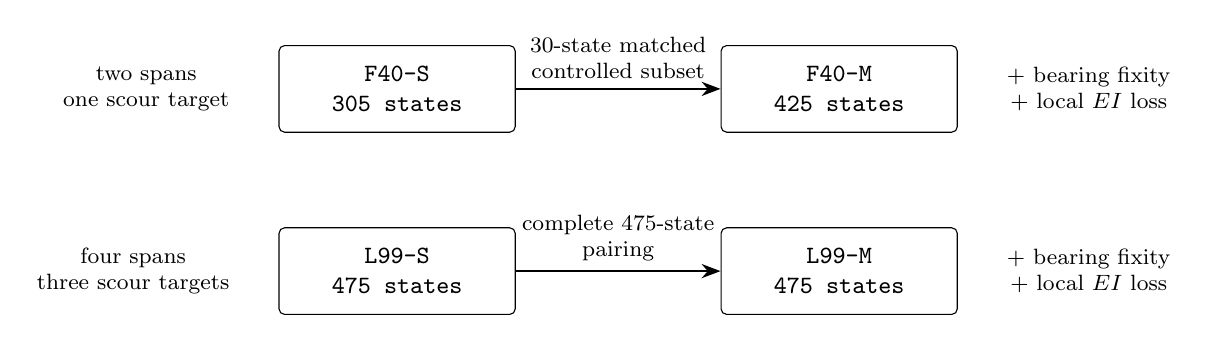
\begin{tikzpicture}[
  node distance=12mm and 26mm,
  block/.style={draw, rounded corners=2pt, minimum height=11mm,
    minimum width=30mm, align=center, font=\small\ttfamily},
  arr/.style={-{Stealth[length=2.4mm]}, thick},
  lbl/.style={font=\footnotesize, align=center}
]
\node[block] (f40s) {F40-S\\305 states};
\node[block, right=of f40s] (f40m) {F40-M\\425 states};
\draw[arr] (f40s) -- node[above,lbl] {30-state matched\\controlled subset} (f40m);
\node[block, below=of f40s] (l99s) {L99-S\\475 states};
\node[block, right=of l99s] (l99m) {L99-M\\475 states};
\draw[arr] (l99s) -- node[above,lbl] {complete 475-state\\pairing} (l99m);
\node[lbl, left=5mm of f40s] {two spans\\one scour target};
\node[lbl, left=5mm of l99s] {four spans\\three scour targets};
\node[lbl, right=5mm of f40m] {+ bearing fixity\\+ local $EI$ loss};
\node[lbl, right=5mm of l99m] {+ bearing fixity\\+ local $EI$ loss};
\end{tikzpicture}%
}
\caption{Four-block Paper-1 design. Arrows denote only authenticated semantic
state pairing; no causal or transport arrow connects the two geometries.}
\label{fig:stage_graph}
\end{figure}

\begin{table}[htbp]
\centering
\caption{Registered Paper-1 scientific blocks. Every state has 50 passages.
One generated FRA-class-4 realization is shared by all states and passages;
speed, temperature, and vehicle properties vary operationally.}
\label{tab:stages}
\small
\setlength{\tabcolsep}{4pt}
\begin{tabular}{llrlp{5.8cm}}
\toprule
Block & Geometry & States & Targets & Expressed bridge mechanisms \\
\midrule
\texttt{F40-S} & $2\times20$ m & 305 & support 2 & scour only; dense 61-severity $\times$ 5-replica grid \\
\texttt{F40-M} & $2\times20$ m & 425 & support 2 & scour + nominal bearing fixity + local $EI$ loss \\
\texttt{L99-S} & $4\times24.9$ m & 475 & supports 2--4 & multi-pier scour only \\
\texttt{L99-M} & $4\times24.9$ m & 475 & supports 2--4 & scour + nominal bearing fixity + local $EI$ loss \\
\bottomrule
\end{tabular}
\end{table}

Track-layer damage, wheel polygonization, and suspension damage remain present
in the single campaign source tree but are disabled by the four stage
configurations; no stripped scientific solver branch is used. Alternative
profile phases are likewise disabled: the production campaign is conditional
on one fixed generated realization. Later track/train-damage or profile-shift
evaluation belongs to a separate study cut from the frozen source revision;
code availability is not evidence that those mechanisms were active in
Paper~1.

\subsection{Execution blocks and provenance}
\label{sec:blocks}

Each scientific block has its own authenticated generation contract,
hyperparameter studies, result manifests, and execution receipts. Training jobs
are distributed through prospectively balanced logical seed partitions, not by
architecture, representation, channel, or observed outcome. The partitions may
run on different capable GPU models and numerical stacks; their exact runtime
identities are recorded as provenance rather than used as equality gates. Each
training PC must pass its own worst-case local capacity probe, and each
generation PC its own capability and physics-smoke suite. Every reported row is
bound to the generating source revision, channel schema, protocol hashes, split
identity, and artifact digests, so that a result without a complete
authenticated lineage fails closed rather than being silently admitted.

\section{Prospective four-block numerical model}
\label{sec:simulation}

This section describes the four-block regression configurations. The completed
F25 classification experiment uses the same solver family with a distinct
39.9~m geometry, 0.15~m deck mesh, stored profile, ten damage classes, and
passage design, as detailed in its dedicated methods section. Four-block
qualification studies below are not F25-specific validation evidence.

\subsection{Train--track--bridge interaction model}
\label{sec:ttbi}

Vehicle responses are generated with a two-dimensional, vertically coupled
train--track--bridge interaction (TTBI) model implemented in MATLAB and derived
from the TTB-2D/VEqMon2D framework of Cantero
\cite{cantero_ttb2d, cantero2022veqmon}. The model couples (i) an
Euler--Bernoulli multi-span deck on vertical support springs and abutment
rotational springs; (ii) a discrete layered track containing rail, pads,
sleepers, ballast, and sub-ballast; and (iii) five identical planar vehicles
with car-body and two-bogie vertical/pitch degrees of freedom and four
constrained unsprung wheelset masses. Vehicle properties follow the
implemented intercity-train calibration attributed to O'Brien et
al.~\cite{obrien2018vehicle}. Wheel--rail interaction is linear and bilateral.
The directly coupled equations are integrated by average-acceleration
Newmark-$\beta$ ($\gamma=1/2$, $\beta=1/4$) at 1~ms.

\paragraph{Implementation provenance.}
The generator is a modified derivative of the published TTB-2D v1 code line,
based on archived upstream commit \texttt{28d35528} and redistributed under
GPL-3.0. The damage mechanisms, campaign catalogues, serialization, and
qualification gates described here are repository-local additions and must not
be attributed to the upstream author. Likewise, the track-property file cites
Zhai et al.~\cite{zhai2004track} and the vehicle file cites O'Brien et
al.~\cite{obrien2018vehicle}; those citations establish the source files'
provenance, not independent validation of every transferred value or topology.

Two bridge geometries are used (Figure~\ref{fig:model}). \textbf{F40} has two
20~m spans and one scour target at the internal support. \textbf{L99} has four
24.9~m spans (99.6~m total) and targets at the three internal supports. The
adopted $E$, $I$, mass per unit length, and 3\% bridge-damping target originate
from the Fernandes two-span example; their use for L99 is an idealized
geometry/scale stress, not calibration of a 99.6~m field bridge. Every state
must pass the registered broad frequency gate and healthy states must reproduce
the nominal healthy first frequency (approximately 4.13~Hz for F40 and
2.75~Hz for L99) within the registered acceptance bands.

\begin{figure}[htbp]
\centering
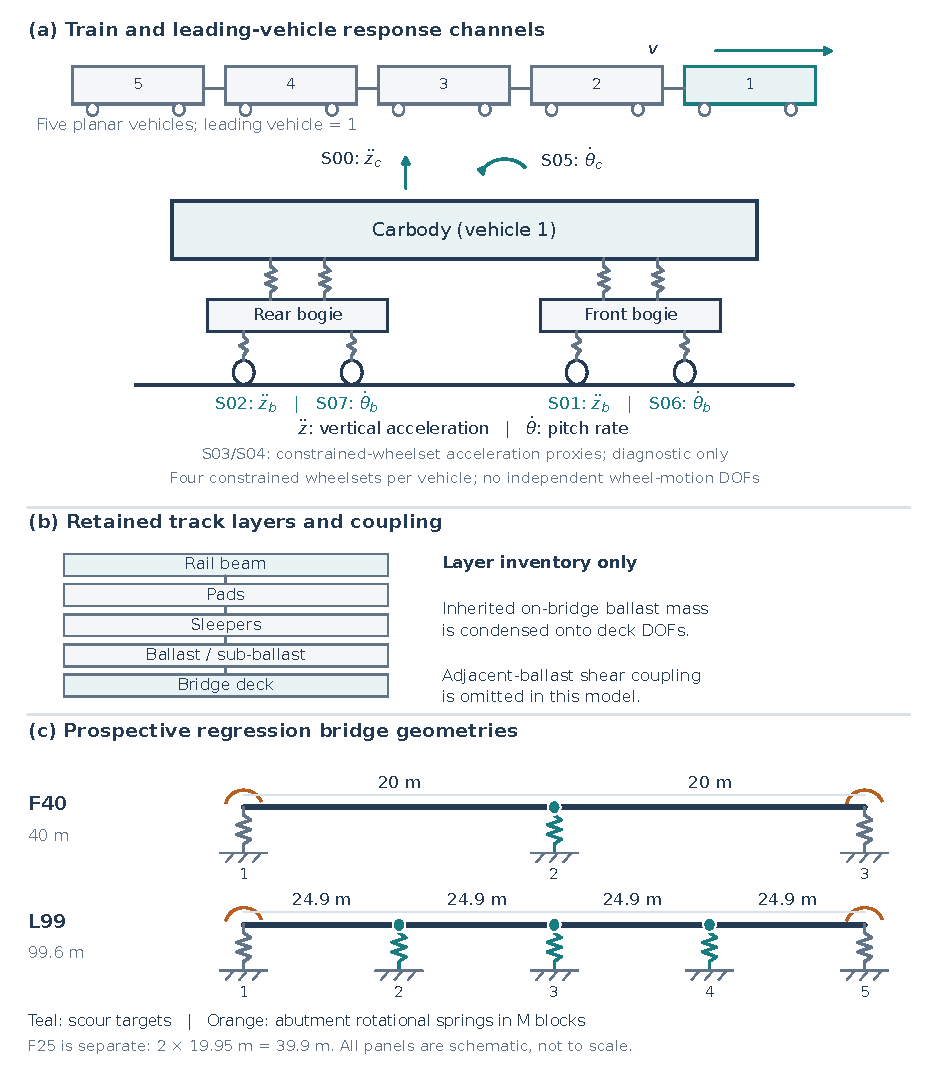
\includegraphics[width=\textwidth]{ttbi_model.pdf}
\caption{Planar TTBI model schematic: (a) five-vehicle train and the six
eligible leading-vehicle responses; constrained-wheelset acceleration proxies
S03/S04 are diagnostic only; (b) retained track-layer inventory and inherited
ballast-condensation boundary; (c) prospective F40/L99 bridge geometries and
scour targets. Orange symbols denote abutment rotational springs in the M
blocks. Not to scale; F25 uses its separate 39.9~m geometry.}
\label{fig:model}
\end{figure}

\subsubsection{Geometry-specific support-aligned meshes}
\label{sec:mesh}

The production meshes are not universally 0.30~m. F40 uses a 0.20~m deck mesh
(three elements per 0.60~m sleeper bay) and a 0.30~m rail mesh (two per bay), so
the internal support is exactly a deck node at 20.0~m. This is a
support-alignment correction to the Fernandes-derived 0.30~m benchmark density:
0.30~m does not divide 20 or 40~m. L99 uses 0.30~m for both deck and rail,
which places all 24.9~m-spaced supports on nodes. Positive support springs are
required to coincide with nodes to roundoff tolerance; they are never snapped
to a nearby grid location.

Production Rayleigh coefficients are recomputed from the first two elastic
modes of each realized bridge state. Mesh-refinement studies independently
recompute the modal references and coefficients on every grid and save the
resulting $\alpha$, $\beta$, and reference modes. A fixed-coefficient arm using
the healthy reference is a sensitivity, not the production closure. Because
the rail-damping matrix uses the corresponding bridge frequencies as its
references, a structural-stiffness intervention in production changes both the
assembled $K$ and Rayleigh-dependent $C$ matrices; it is not evidence that
physical damage itself changes damping.

\subsubsection{Finite rail-domain selection}
\label{sec:rail_clearance}

The finite rail domain was selected by the source-locked 18-case matrix recorded
in \nolinkurl{docs/evidence/paper1_model_form_freeze_20260809.json}. The
production decision identifier is
\nolinkurl{paper1-rail-domain-clearance-c06-v1}.
For each of F40 and L99, the matrix crossed three operating points
$(70~\mathrm{km/h},3\,^{\circ}\mathrm{C})$,
$(80~\mathrm{km/h},18\,^{\circ}\mathrm{C})$, and
$(90~\mathrm{km/h},33\,^{\circ}\mathrm{C})$ with 6, 15, and 30~m clearances.
All 18 cases completed. Both registered comparison tiers --- C06 versus C30
and C15 versus C30 --- passed, so the rule selected 6~m for production. The
verdict is bound to generator source-root SHA-256
\texttt{aa187204cb3f89e2\allowbreak4cb8bc894034044b\allowbreak%
ad38b0358f5e0cd5\allowbreak86338f84a8418efb}.
Its supported claim is strictly finite-rail-domain selection for this
source-locked case matrix; it is not general mesh/time-step convergence,
damage-model validation, or physical/field validation.

\subsubsection{Track-property and topology boundary}
\label{sec:track_boundary}

The implemented nominal track is an inherited hybrid planar convention, not a
blanket sum of all Zhai quantities into two rails. Zhai et
al.~\cite{zhai2004track} report their Table~1 quantities per rail seat at
0.545~m spacing. The implementation doubles rail inertia and rail mass and uses
a full sleeper mass, but retains the tabulated pad, ballast, and sub-ballast
terms at one-seat values. It then places those values on a 0.600~m sleeper
lattice without re-evaluating the spacing-dependent $M_b$, $K_b$, and $K_f$
expressions. The production baseline is therefore neither a demonstrated
one-seat line model nor a consistently doubled two-rail equivalent.

The topology is also simplified relative to Zhai: adjacent-ballast shear
couplings $K_w,C_w$ are omitted, and the complete retained ballast mass is
condensed onto the support-aligned deck degree of freedom at every on-bridge
sleeper. This is an explicit inherited model-form choice. The topology arm was
dropped because it would require new solver structure and is not examined in
this paper.

Three parameter-level sensitivity families are prospectively fixed against the
hybrid baseline: (i) consistent one-seat and consistent two-rail scaling;
(ii) recomputation of $M_b$, $K_b$, and $K_f$ at 0.600~m from Zhai's equations;
and (iii) 0.050\% and 0.200\% rail-damping targets around the inherited 0.100\%
target. The 0.100\% target is author-chosen and is not reported by Zhai.
Sensitivity outcomes qualify interpretation but do not silently redefine the
production model after its source freeze.

\begin{table}[htbp]
\centering
\caption{Nominal physical and numerical parameters read from the implemented
baseline. Track entries preserve the hybrid scaling and topology described in
Section~\ref{sec:track_boundary}; they must not be labeled uniformly
``two-rail Zhai values''.}
\label{tab:parameters}
\footnotesize
\setlength{\tabcolsep}{4pt}
\resizebox{\textwidth}{!}{%
\begin{tabular}{llll}
\toprule
Subsystem & Parameter & Value & Units \\
\midrule
\multirow{8}{*}{Bridge}
 & spans (F40 / L99) & $2\times20$ / $4\times24.9$ & m \\
 & Young's modulus $E$ at 15\,$^{\circ}$C & $35\times10^{9}$ & N/m$^2$ \\
 & second moment of area $I$ & 0.33 & m$^4$ \\
 & mass per unit length & 9600 & kg/m \\
 & Rayleigh target, first two elastic modes & 3 & \% \\
 & healthy vertical support stiffness $k_{v,0}$ & $3.44\times10^{8}$ & N/m \\
 & free-rotation abutment baseline & 0 & N$\cdot$m/rad \\
 & healthy first frequency (F40 / L99) & $\approx4.13$ / $\approx2.75$ & Hz \\
\midrule
\multirow{8}{*}{Track}
 & rail bending stiffness $EI$ & $1.325\times10^{7}$ & N$\cdot$m$^2$ \\
 & rail mass (doubled-rail entry) & 121.28 & kg/m \\
 & rail Rayleigh target (inherited) & 0.100 & \% \\
 & pad stiffness / damping (one-seat entry) & $6.5\times10^{7}$ / $7.5\times10^{4}$ & N/m, N$\cdot$s/m \\
 & sleeper spacing / full mass & 0.600 / 251 & m, kg \\
 & ballast mass / stiffness / damping (one-seat entries) & 531.4 / $1.3775\times10^{8}$ / $5.88\times10^{4}$ & kg, N/m, N$\cdot$s/m \\
 & sub-ballast stiffness / damping (one-seat entries) & $7.75\times10^{7}$ / $3.115\times10^{4}$ & N/m, N$\cdot$s/m \\
 & finite rail clearance beyond deck & 6 & m \\
\midrule
\multirow{7}{*}{Vehicle ($\times5$)}
 & car-body mass / pitch inertia & 36852 / 560342 & kg, kg$\cdot$m$^2$ \\
 & bogie mass / pitch inertia & 3910 / 10024 & kg, kg$\cdot$m$^2$ \\
 & wheelset mass & 1407 & kg \\
 & primary suspension stiffness / damping per axle & $5.558\times10^{6}$ / $5.88\times10^{4}$ & N/m, N$\cdot$s/m \\
 & secondary suspension stiffness / damping per bogie & $2.0\times10^{6}$ / $1.2\times10^{5}$ & N/m, N$\cdot$s/m \\
 & bogie-centre / axle spacing & 16 / 2.3 & m \\
 & vehicle length / wheel radius & 22 / 0.46 & m \\
\midrule
\multirow{4}{*}{Solver}
 & integration & Newmark-$\beta$ ($\gamma=1/2$, $\beta=1/4$) & --- \\
 & time step / stored rate & $10^{-3}$ / 1000 & s, Hz \\
 & deck element (F40 / L99) & 0.20 / 0.30 & m \\
 & rail element (F40 / L99) & 0.30 / 0.30 & m \\
\bottomrule
\end{tabular}%
}
\end{table}

\subsection{Response-channel schema}
\label{sec:response_channels}

The leading vehicle supplies the eight stored responses in
Table~\ref{tab:channels}, identified collectively as
\texttt{physical8\_v1}. Six are direct responses of modeled car-body/bogie
degrees of freedom and constitute the complete learning-eligible set. The
other two are the total vertical accelerations implied
by the constrained motion of the first two wheelsets,
\begin{equation}
  \ddot z_w = u_{,tt} + 2v\,u_{,xt} + v^2 u_{,xx} + \ddot h_w,
  \label{eq:wheelset_proxy}
\end{equation}
where $u$ is the rail displacement field evaluated along the moving contact
coordinate, $v$ is passage speed, and $h_w$ is the prescribed profile/wheel
path. These two rows are idealized, model-predicted
\emph{constrained-wheelset acceleration proxies}. They are kinematic
diagnostics, not independent wheelset degrees of freedom, not the Eulerian
rail-field acceleration $u_{,tt}$ alone, and not validated measurements from
axle-box sensors. Payload indices 3 and 4 are excluded from all learning,
screening, and pair selection.
The separate stored \texttt{acc\_under} rows remain virtual rail-field
diagnostics and never enter the six-channel eligible learning screen.

\begin{table}[htbp]
\centering
\caption{Stored \texttt{physical8\_v1} responses of the leading vehicle.}
\label{tab:channels}
\small
\begin{tabular}{cll}
\toprule
Index & Response channel & Observation status \\
\midrule
0 & car-body vertical acceleration & modeled secondary-suspended DOF \\
1 & front-bogie vertical acceleration & modeled primary-suspended DOF \\
2 & rear-bogie vertical acceleration & modeled primary-suspended DOF \\
3 & wheelset-1 constrained vertical acceleration & diagnostic-only kinematic proxy \\
4 & wheelset-2 constrained vertical acceleration & diagnostic-only kinematic proxy \\
5 & car-body pitch angular velocity & modeled secondary-suspended DOF \\
6 & front-bogie pitch angular velocity & modeled primary-suspended DOF \\
7 & rear-bogie pitch angular velocity & modeled primary-suspended DOF \\
\bottomrule
\end{tabular}
\end{table}

The proxy label is deliberate. Equation~\eqref{eq:wheelset_proxy} omits a
hardware observation chain, local axle-box mounting dynamics, sensor bandwidth
and filtering, and contact nonlinearity. Accordingly, the channel screen ranks
only the six modeled-DOF responses (indices 0, 1, 2, 5, 6, and 7). The two
proxies remain available for physical diagnostics but cannot determine a
learning input, transducer count, or procurement choice.

\subsubsection{Contact-model scope and qualification}
\label{sec:contact}

The bilateral linear contact model does not simulate separation and re-contact.
Wheel flats and polygonization are disabled in all four Paper-1 blocks. Every
retained passage nevertheless carries finite/contact diagnostics and fails
generation if it violates the registered admissibility contract. Before
retained production, the source-level contact-closure study evaluates all 420
passages of the four
marked qualification datasets at 1.0, 0.5, and 0.25~ms, applies the registered
0/12/24~kN tension gates and 0.002 path-fraction gate, and checks waveform and
quantity-of-interest convergence. This is an engineering consistency gate for
the finite design, not validation of bilateral contact physics.

\subsection{Active bridge mechanisms}
\label{sec:mechanisms}

\subsubsection{Scour as support-stiffness loss}
\label{sec:scour_mech}

At each target support, scour is represented as
\begin{equation}
  k_v(d)=(1-d)k_{v,0}, \qquad 0\le d\le0.60,
  \label{eq:scour}
\end{equation}
with $k_{v,0}=3.44\times10^8$~N/m. The regression label is $100d$,
modeled support-stiffness loss in percentage points. This follows the
drive-by-scour convention~\cite{fernandes2024driveby,
fernandes2025early, prendergast2013investigation}, but is not scour depth,
embedment loss, or eroded volume.

\subsubsection{Nominal bearing fixity}
\label{sec:bearing_mech}

F40-M and L99-M activate a rotational spring at each abutment. The sampled
geometry-normalized coordinate is
\begin{equation}
 \varphi=\frac{k_r}{k_r+4E_{15}I/L_{\mathrm{end}}}
 \quad\Longleftrightarrow\quad
 k_r=\frac{\varphi}{1-\varphi}\frac{4E_{15}I}{L_{\mathrm{end}}},
 \qquad \varphi\in[0,0.95].
 \label{eq:fixity}
\end{equation}
The stiffness is computed once using the fixed 15\,$^{\circ}$C modulus and
remains constant while the deck modulus varies between passages. The two
fixity coordinates are additional M-block regression targets. They are nominal
free-to-near-fixed design variables, not calibrated bearing-damage percentages
or physical seizure thresholds.

\subsubsection{Local flexural-rigidity-loss surrogate}
\label{sec:crack_mech}

F40-M and L99-M reduce $EI$ uniformly over the single production finite element
containing the sampled damage location, with author-chosen severity
$\mathcal{U}(0.05,0.30)$. Locations use an author-chosen 4:1 design weighting
toward hogging regions inside the registered support-zone and bridge-length
bounds. No fitting dataset supports those occurrence or severity laws. The
damaged length is consequently one mesh-locked element --- 0.20~m on F40 and
0.30~m on L99 --- rather than a common physical crack length. This is a local
damaged-element benchmark, not the tapered crack-depth model of Sinha et
al.~\cite{sinha2002simplified}; its severity is never interpreted as crack
depth. Crack status is logged but not predicted.

\subsection{Fixed profile, operational variability, and deferred mechanisms}
\label{sec:opvar}

Every state and passage in all four blocks uses one generated realization of
the implemented FRA-class-4 vertical-profile spectrum (registered phase seed
20260728). No measured profile, per-state phase variation, or per-passage
profile jitter is used. The fixed choice controls excitation geometry across
healthy/damaged states and matched S--M comparisons.

Operational conditions do vary. Each state's 50 passages use a Latin
hypercube over speed 70--90~km/h and temperature 3--33~$^{\circ}$C, rounded to
integer values. Temperature changes the deck modulus through the registered
author-chosen law
\[
 E(T)=E_{15}\,[1-0.003(T-15)].
\]
For each passage and vehicle, car-body mass has a 10\% Gaussian coefficient of
variation and primary/secondary suspension stiffnesses each have 5\%. These
envelopes and laws were not fitted to a route, climate, or fleet population.

Track-layer damage (ballast patches, hanging sleepers, and pad failure), wheel
polygonization, suspension damage, and alternative rail-profile phases are
disabled by all four stage contracts. The corresponding code remains in the
single source tree for future work; it contributes no expressed physics or
random variability to Paper~1.

\subsection{State catalogues and common random numbers}
\label{sec:states}

Table~\ref{tab:families} gives the exact state inventories. F40-S is a dense
61-severity grid (0--60\% in one-percentage-point increments) with five
semantic replicas per severity. F40-M uses five controlled families. Its five
healthy replicas and five replicas at each of 12, 24, 36, 48, and 60\% scour
form the exact 30-state subset shared with F40-S. L99-S and L99-M share their
complete five-family, 475-state latent design; bearing/crack coordinates are
dormant in L99-S rather than being removed or redrawn.

\begin{table}[htbp]
\centering
\caption{Registered state families. Every state has 50 operational passages.}
\label{tab:families}
\small
\begin{tabular}{lrrrp{5.0cm}}
\toprule
Family & F40-S & F40-M & L99-S/M & Role \\
\midrule
\texttt{target\_healthy} & 5 & 50 & 50 & zero-scour diagnostic \\
\texttt{scour\_only} & 300 & 25 & 75 & controlled support/severity anchors \\
\texttt{bearing\_only} & 0 & 50 & 50 & bearing/leakage anchors; dormant in L99-S \\
\texttt{nuisance\_only} & 0 & 50 & 50 & local-$EI$ anchors; dormant in L99-S \\
\texttt{joint} & 0 & 250 & 250 & multivariate latent design \\
\midrule
Total & 305 & 425 & 475 & \\
\bottomrule
\end{tabular}
\end{table}

Each state has a collision-checked semantic \texttt{StateUID}. Named substreams
derive operational, crack, track, and reserved passage/profile identities from
that UID rather than a mutable row number or parallel-execution order. The
production profile does not consume the state-keyed phase identity: its global
phase comes from registered seed 20260728. Only streams for expressed Paper-1
mechanisms influence the solve; disabled profile/track/wheel namespaces remain
inert. States are the split and resampling clusters, and their 50 passages are
correlated repeated observations, not independent field samples.

The generator stores raw noise-free histories, semantic identities, latent
design coordinates, operational draws, profile and model-form identifiers,
modal/Rayleigh records, contact diagnostics, crop metadata, and source-bound
fingerprints. Observation noise is added only by the authenticated learning
pipeline (Section~\ref{sec:preprocessing}).

\section{Prospective regression methods}
\label{sec:data_processing}

The methods in this section apply to the prospective F40/L99 regression
campaign. F25 classification instead uses its separately specified
class-stratified passage split, Min--Max scaling, PAA-583 representation,
noise equation, search protocol, and 20-seed reporting design. Its observed
results must be interpreted under those dedicated methods.

\subsection{From generated responses to model inputs}
\label{sec:preprocessing}

\paragraph{Time-to-space transformation.}
Raw time histories are linearly interpolated onto a uniform spatial grid of
100 samples per metre and cropped to the registered bridge-centred window.
Speed is constant within a passage, so the time--space map is affine. This
aligns each bridge support and its response signature at the same input
location despite passage-speed variation.

\paragraph{RAW and PAA representations.}
The factorial compares the cropped spatial sequence directly (RAW) with true
Piecewise Aggregate Approximation (PAA) to 512 segments
\cite{keogh2001dimensionality}. PAA partitions the sequence into equal-width
windows and replaces each by its mean, with fractional boundaries handled
exactly. It is therefore both a dimensionality-reduction and low-pass
compression front end. Its inclusion follows drive-by damage-classification
precedent~\cite{fernandes2025early}; no universal denoising advantage is
assumed. RAW and PAA use the same downstream model interfaces.

\paragraph{Observation-noise stress.}
The main observation arm adds pointwise zero-mean Gaussian multiplicative
noise with standard deviation $0.05|x|$ after the space transform and crop but
before PAA and scaling. The generator is keyed by global channel index, so a
channel receives the same noise realization when evaluated alone or in any
pair. This is a symmetric mathematical stress, not a sensor model: it contains
no transducer-specific noise density, bias, bandwidth, mounting transfer
function, or environmental qualification~\cite{en61373}.

\paragraph{Per-channel scaling.}
A per-channel affine standardization is fitted on training states only and
applied unchanged to validation and test data. Fold-level adjudication refits
the scaler within each fold-training partition. No scaler sees its validation
fold or the sealed outer test.

\subsection{Learning tasks}
\label{sec:task}

The primary task is continuous multi-output regression. F40-S and F40-M have
one scour head for support~2; L99-S and L99-M have one scour head for each of
supports 2--4. The M blocks additionally contain one nominal-fixity head for
each abutment. Scour targets span 0--60 percentage points and fixity targets
0--95. The M-block training loss is a range-normalized multi-head MSE with
weights proportional to the inverse squared target range and normalized to
mean one. Selection remains scour-primary; bearing error and
scour--bearing leakage are secondary diagnostics. F40-S also supplies a
predeclared four-class subset at 0, 5, 10, and 20\% modeled stiffness loss for
a secondary Fernandes-style comparability check.

\subsection{Factorial architecture grid}
\label{sec:architectures}

The architecture experiment is the complete
\[
  \{\mathrm{RAW},\mathrm{PAA}\}
  \times\{\mathrm{position\ off,on}\}
  \times\{\mathrm{LSTM\ off,on}\}
  \times\{\mathrm{multi\!\mbox{-}\!rate\ off,on}\},
\]
giving 16 cells. All cells share a one-dimensional convolutional backbone and
dense regression heads; the three binary components have these meanings:

\begin{itemize}
  \item \textbf{Time2Vec-style spatial-coordinate encoding.} One linear and
  seven learnable sinusoidal functions of normalized bridge position are
  concatenated to the input, following the Time2Vec construction
  \cite{kazemi2019time2vec} on a spatial rather than temporal coordinate. The
  implementation is not a full Space2Vec model~\cite{mai2020space2vec}.
  \item \textbf{LSTM recurrence.} A unidirectional LSTM
  \cite{hochreiter1997long} follows the convolutional backbone, motivated by
  CNN--LSTM precedent in drive-by scour classification
  \cite{fernandes2026canelas}.
  \item \textbf{Fixed-width multi-rate pooling.} Parallel adaptive temporal
  pyramid branches summarize several registered rates and concatenate a fixed
  number of features. The output width and dense parameter count do not depend
  on RAW/PAA sequence length. The module is inspired by the multi-rate idea in
  N-HiTS~\cite{challu2023nhits}, but it is not the N-HiTS forecasting
  architecture: it has no backcast/forecast stacks or hierarchical
  interpolation.
\end{itemize}

The cell with all three components off is the CNN--global-average-pooling
(CNN--GAP) baseline within each representation. The factorial estimates
matched finite-design component contrasts, but does not prove that a component
is universally beneficial outside the registered search spaces and budget.

\begin{figure}[htbp]
\centering
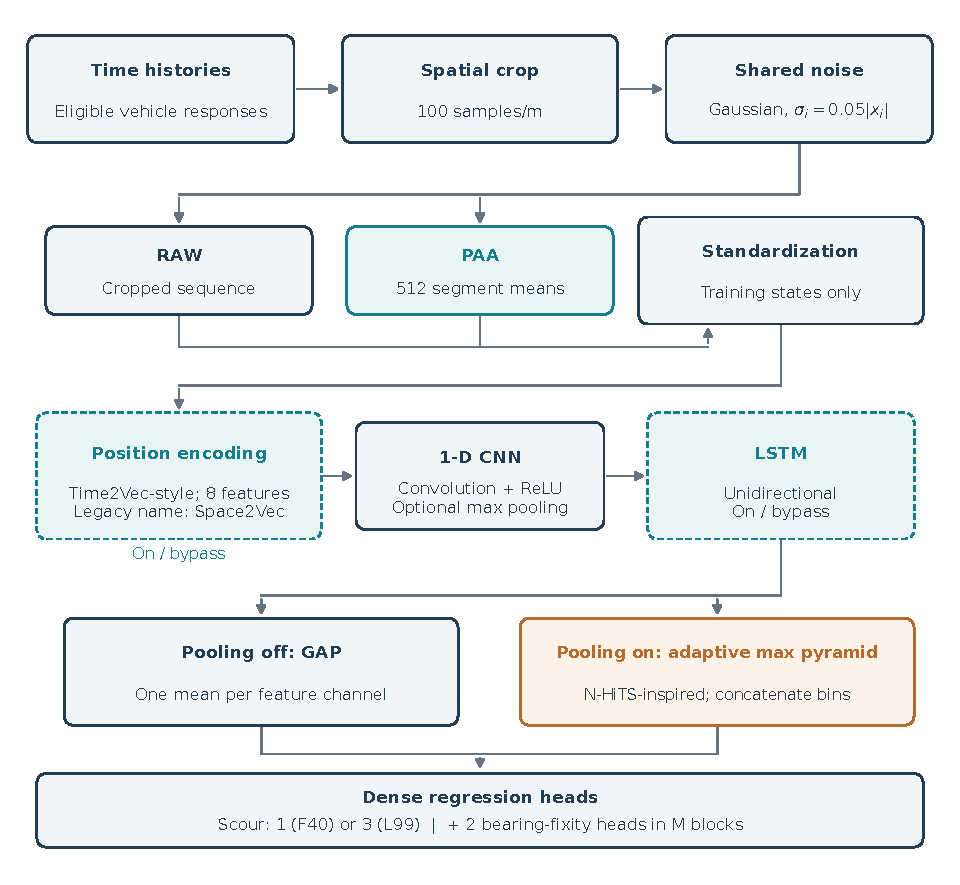
\includegraphics[width=\textwidth]{regression_architecture.pdf}
\caption{Processing chain and prospective 16-cell regression architecture
grid. RAW/PAA inputs are standardized using training states only. Optional
spatial-coordinate encoding (legacy Space2Vec) and LSTM precede global-average
or N-HiTS-inspired adaptive pyramid pooling and the block-specific dense
regression heads. Dashed boxes denote components that can be bypassed.
These prospective cells are separate from the executed F25 classifier arms.}
\label{fig:architectures}
\end{figure}

\begin{table}[htbp]
\centering
\caption{Registered continuous hyperparameter-search domains shared across
eligible cells; conditional domains appear only when their component is on.}
\label{tab:search_space}
\small
\begin{tabular}{lll}
\toprule
Scope & Hyperparameter & Domain \\
\midrule
base & convolutional layers & integer 2--4 \\
base & dense layers & integer 1--3 \\
base & learning rate & log-uniform $10^{-4}$--$10^{-2}$ \\
base & weight decay & log-uniform $10^{-5}$--$10^{-3}$ \\
per convolution & filters / kernel / max-pooling & 16--128 step 16 / $\{2,3,5,7\}$ / off,on \\
per dense layer & units / dropout & 32--256 step 16 / 0.1--0.5 \\
LSTM on & layers / hidden width / dropout & 1--2 / 32--128 step 32 / 0.1--0.4 \\
multi-rate on & adaptive-pyramid rate set & $\{(1,2,4),(1,4,8),(1,3,6),(1,2,4,8)\}$ \\
\bottomrule
\end{tabular}
\end{table}

Every trial uses batch size 32, at most 50 epochs, early-stopping patience 5,
Adam~\cite{kingma2015adam}, and cosine learning-rate annealing
\cite{loshchilov2017sgdr}. Failed trials, retries, out-of-memory events, and
incomplete terminal accounting fail the publication contract.

\subsection{State-grouped split and sealed-test firewall}
\label{sec:split}

Structural states are assigned by semantic identity to a deterministic split:
60\% for training, 20\% for inner validation, and 20\% for the outer test
(split seed 42). All 50 passages of one state remain together. Each controlled
cell assigns its five semantic replicas 3/1/1 to these partitions. Joint-state
strata preserve the specified severity and nuisance balance. States paired
across blocks receive the same assignment. The outer test stays sealed during
factorial HPO, development adjudication, channel screening, and selected-pair
HPO.

\subsection{F40-S factorial HPO and Option-C adjudication}
\label{sec:hpo}

The prospectively chosen HPO input is channel~1, front-bogie vertical
acceleration. On F40-S, each of the 16 cells receives five independent Optuna
restarts~\cite{akiba2019optuna} of 100 trials with the registered TPE sampler
\cite{bergstra2011algorithms} and successive-halving pruner
\cite{jamieson2016non}: 80 studies and 8,000 requested trials.

The best vector from each restart is then adjudicated by Option~C on one
prospectively fixed grouped-development OOF partition (seed 271828,
$n_{\mathrm{splits}}=3$, one repeat). Every candidate is refitted on folds
0--2 with initialization seeds 424243 and 8675309. Thus each cell has
$5\times3\times2=30$ fits and the factorial has 480. For every
candidate/initialization pair, the three validation folds are disjoint and
cover each development state exactly once. Scour MSE is first averaged across
the two initialization seeds within each state and then equally across states.
The minimum selects the vector; an exact tie selects the lowest HPO-restart
seed. The best RAW and PAA cells are their respective minimum-score cells, with
lexicographic cell identifier as the tie-break. These 480 fits are a selection
mechanism, not a post-selection stability estimate.

Four pipeline slots are retained: the best RAW cell, the best PAA cell, and the
RAW and PAA CNN--GAP baselines. If a winner is its representation's baseline,
the authenticated alias is deduplicated rather than treated as an independent
pipeline.

\subsection{Prospectively fixed response-channel screen}
\label{sec:channel_design}

The F40-S payload contains the eight \texttt{physical8\_v1} responses in
Table~\ref{tab:channels}, but learning eligibility is restricted to the six
modeled-DOF responses at indices 0, 1, 2, 5, 6, and 7. Wheelset-proxy indices 3
and 4 remain diagnostic-only and are excluded from every training and selection
input. For each retained slot, the screen evaluates the six eligible singles
and all $\binom{6}{2}=15$ ascending eligible pairs at the adjudicated frozen
hyperparameters and checkpoint epoch, using paired initialization seeds
4001, 4003, 4007, 4013, and 4019. The prospectively enumerated grid therefore
contains $4\times21\times5=420$ job slots before authenticated alias
deduplication; a winner/baseline alias is not retrained as though it were a
distinct pipeline. Each fit uses the canonical train-to-inner-validation
grouped partition; the outer test remains sealed.

For one input/pipeline, per-state scour MSE is averaged over the five seeds and
then equally across validation states. The input score is then averaged equally
over unique resolved pipelines. Singles are reported diagnostics but cannot
select. The minimum among the 15 pairs wins, with lexicographic ascending-pair
tie-breaking. The artifact authenticates the full result tensor, state
coverage, and deduplication map; no result-dependent pair can be inserted.

\subsection{Selected-pair HPO, stability, and secondary transfer}
\label{sec:post_selection}

After pair selection, each of the four retained slots receives five new
100-trial searches on that pair in F40-S. The same four slots receive
independent five-by-100-trial selected-pair HPO in F40-M, L99-S, and L99-M.
This contributes another 80 studies and 8,000 requested trials. Together with
the factorial anchor, the primary registered HPO budget is exactly 160 studies and
16,000 trials. There is no transport gate, no rescue trigger, and no primary
downstream result based on inherited F40-S hyperparameters.

Only after the primary F40-S screen authenticates its selected pair may the
optional ModernTCN- and TSLANet-inspired contemporary challengers enter. Every
challenger receives that same pair; none may train on the diagnostic proxy rows,
run an independent channel screen, or select a different pair. This secondary
tier is outside the primary 16-cell selection and the primary accounting below.

After each block's vectors and checkpoint policy are frozen, four slots are
trained on the complete development set with 30 disjoint prospectively listed
initialization seeds and evaluated on the sealed outer test: $4\times4\times
30=480$ report-only stability fits. They cannot re-rank the selected models.
A separate secondary analysis applies frozen F40-S settings to the three
downstream blocks with four slots and five seeds ($3\times4\times5=60$ fits).
It is descriptive/non-selection only. The complete prospective refit grid is
480 adjudication + 420 channel-screen + 480 stability + 60 transfer = 1,440
listed fits, subject only to authenticated alias deduplication.

\subsection{Evaluation and registered analyses}
\label{sec:metrics}

Primary block tables report scour MSE in squared percentage points, aggregate
and per support, with RMSE where useful. Multi-pier blocks additionally report
the passage-level most-affected-support localization accuracy for passages
whose maximum true scour is strictly above 5 percentage points. M blocks report
bearing-head MSE, false scour response in bearing-only states, and false
bearing response in scour-only states. Seed distributions and state-first
resampling summaries are reported as descriptive finite-design sensitivity,
not population confidence intervals.

The two paired S--M analyses use only identical sealed-test StateUIDs and a
fixed paired seed axis. Within a seed, scour MSE is averaged equally over
eligible states; the registered point statistic is the median across the finite
seed list. One hundred thousand paired state-first bootstrap draws (seed 42;
the seed axis is never resampled) provide a pointwise descriptive interval and
a wider two-comparison tail-adjusted envelope. Neither has population coverage
or familywise-error-control semantics. F40 uses its exact 30-state shared
subset; L99 uses all 475 shared states.

\subsection{Reproducibility and provenance}
\label{sec:reproducibility}

Generation records the actual MATLAB numerical-stack descriptor, and learning
records the actual Python/PyTorch/CUDA stack and GPU identity. The reviewed
descriptors are known-good setup references, but exact version equality is not
an eligibility condition. Source roots, generation contracts, channel schema,
split identity, study identities, weights, scalers, selection artifacts, and
execution receipts are content authenticated and cross-checked at resume and
analysis boundaries. Every generation PC must pass its local capability and
healthy/damaged physics-smoke suite; the source-level contact gate covers all
420 marked qualification passages. Every training PC must additionally pass a
genuine worst-case two-channel CUDA capacity preflight. Cross-release comparison
and timing benchmarks are optional diagnostics. These checks provide artifact
integrity and internal consistency under a trusted-operator model; they are not
cryptographic hardware attestation.

\section{F25 benchmark: reconstruction and extension of Fernandes et al.\ (2025)}
\label{sec:f25_methods}

This section describes the completed classification study. F25-R reconstructs
the ten-class multi-damage benchmark of Fernandes et
al.~\cite{fernandes2025early} with its two original response channels; F25-X
extends it to six vehicle responses and to a CNN with multi-rate pooling. Both
use the same simulated passages, data partition, measurement noise, and
initialization seeds, so their differences are not affected by resampling of
the dataset. F25 is a classification study of ten fixed damage scenarios. It is
independent of the regression campaign described in
Sections~\ref{sec:framework}--\ref{sec:data_processing} and provides none of
its outcomes.

\subsection{Bridge model and damage scenarios}

The bridge is the two-span railway viaduct of the source study: an
Euler--Bernoulli beam with $E=35$~GPa at 15~$^{\circ}$C, $I=0.33$~m$^4$, a mass
of 9,600~kg/m, and 3\% Rayleigh damping, crossed by the five-vehicle train and
layered track of Section~\ref{sec:ttbi}. The source text describes two 20~m
spans, whereas its finite-element grid of 133 elements of 0.30~m corresponds to
a 39.9~m deck with two 19.95~m spans; the latter geometry is reproduced here.
The deck is discretized into 266 elements of 0.15~m. This uniform refinement
keeps every node of the source grid and places the central support, which lies
inside an element of the source grid, on a node. The healthy vertical stiffness
of the central support is $k_v=3.44\times10^{8}$~N/m, and both end bearings are
free to rotate~\cite{fernandes2025early}.

Table~\ref{tab:f25_scenarios} lists the ten scenarios. Scour is represented by a
5\% or 10\% reduction of $k_v$. Bearing damage is represented by a rotational
stiffness of $10^{9}$~N\,m/rad at the entrance bearing. The source models a
crack with the tapered flexural-rigidity law of Sinha et
al.~\cite{sinha2002simplified}, located at the mid-span of the second span, and
reports that crack-depth ratios of 0.10 and 0.05 correspond to $EI$ reductions
of approximately 22\% and 14\% for a 0.30~m element. Here those reductions are
applied uniformly over the same 0.30~m zone, $29.70\le x\le30.00$~m, which
consists of two refined elements. The crack-depth ratios are kept as class
labels; they are not depths calibrated for the uniform surrogate.

\begin{table}[htbp]
\centering
\caption{Damage scenarios of the F25 benchmark~\cite{fernandes2025early}. The
crack label is the source crack-depth ratio; the simulated intervention is the
listed uniform $EI$ reduction. Bearing damage denotes the rotational restraint
of the entrance bearing.}
\label{tab:f25_scenarios}
\small
\begin{tabular}{lrrrc}
\toprule
Scenario & Crack label (\%) & $EI$ reduction (\%) & Scour, $k_v$ reduction (\%) & Bearing damage \\
\midrule
Healthy & 0 & 0 & 0 & -- \\
DC2 & 10 & 22 & 0 & -- \\
DC3 & 0 & 0 & 5 & -- \\
DC4 & 0 & 0 & 0 & yes \\
DC5 & 0 & 0 & 10 & yes \\
DC6 & 10 & 22 & 10 & -- \\
DC7 & 10 & 22 & 0 & yes \\
DC8 & 10 & 22 & 10 & yes \\
DC9 & 10 & 22 & 5 & yes \\
DC10 & 5 & 14 & 5 & yes \\
\bottomrule
\end{tabular}
\end{table}

\subsection{Operational variability and simulated measurements}

Each scenario is simulated for 200 passages, giving 2,000 passages. For each
scenario a Latin hypercube~\cite{mckay1979comparison} of 17 variables is drawn:
the train speed (70--90~km/h), the temperature (3--33~$^{\circ}$C), and, for each
of the five vehicles, the carbody mass (33,000--40,000~kg) and the primary and
secondary suspension stiffnesses (2,640--2,920 and 942--1,042~kN/m per side,
doubled in the planar model). These are the ranges of the source
study~\cite{fernandes2025early}. Temperature modifies the deck modulus as
$E(T)=E_{15}\,[1-0.003\,(T-15)]$. The rail profile is the stored FRA class-4
realization used by Fernandes et al.~\cite{fernandes2024driveby,
fernandes2025early}; it is the same for every passage and scenario and differs
from the generated realization adopted for the regression campaign. Every
passage satisfied the wheel--rail contact admissibility check of the solver.

Following the source, the responses of the leading vehicle are monitored while
its axles cross the bridge, approximately from the entry of the first axle to
the exit of the last one, and are resampled at 100 samples/m. The source reports
a 58.3~m window of 5,830 samples. Its window convention, which uses a 40~m
bridge term, yields 5,831 inclusive samples on the present grid, and the last
sample is discarded. The resulting window is nine samples (0.09~m) longer than
a window computed with the exact 39.9~m deck length.

\subsection{Data partition, measurement noise, and preprocessing}

The passages of each scenario are split into 80 training, 20 validation, and
100 test passages, as in the source. The allocation is a single random
permutation of the local passage indices (PCG64 generator, seed 2025080901),
applied identically to all scenarios and all configurations; the training,
validation, and test sets therefore contain 800, 200, and 1,000 passages. Each
scenario corresponds to one fixed structural configuration, so this split
measures the recognition of known configurations under new operational
conditions, not generalization to unseen damage states.

Measurement noise follows Eq.~(2) of the source~\cite{fernandes2025early}:
\begin{equation}
    x^{\mathrm{noisy}}_i=x_i+0.05\,\sigma(x)\,\epsilon_i,
    \qquad \epsilon_i\sim\mathcal{N}(0,1),
    \label{eq:f25_noise}
\end{equation}
where $\sigma(x)$ is the standard deviation of the clean signal $x$ of one
passage and channel. One noise realization is generated for each scenario,
passage, and channel and is shared by all representations and models. Each
channel is then min--max normalized,
\begin{equation}
    \tilde{x}_i=\frac{x_i-x_{\min}}{x_{\max}-x_{\min}},
\end{equation}
with $x_{\min}$ and $x_{\max}$ computed on the training set only and applied
without clipping to the validation and test sets. RAW inputs keep all 5,830
normalized samples. PAA inputs~\cite{keogh2001dimensionality} replace each
block of ten consecutive samples by its mean, giving 583 values per channel, the
segment length selected in the source study.

\subsection{Response channels}

Six responses of the leading vehicle are considered (Fig.~\ref{fig:model}a):
the vertical accelerations of the carbody (S00), front bogie (S01), and rear
bogie (S02), and the pitch rates of the carbody (S05), front bogie (S06), and
rear bogie (S07). F25-R uses S00 and S01, the carbody and front-bogie sensors of
the source study, each as a single input. F25-X considers all six single
channels and all 15 two-channel combinations. Wheelset accelerations are not
used: in the planar model the wheelsets follow the rail, so their accelerations
are kinematic quantities rather than independent responses
(Section~\ref{sec:response_channels}).

\subsection{CNN architectures}

RAW-CNN and PAA-CNN reproduce the source architecture
(Fig.~\ref{fig:f25_architecture}): one to five valid one-dimensional
convolutions with ReLU activation, each optionally followed by max pooling of
size two, a flatten layer, a dense ReLU layer, and a ten-class output layer.
PAA-MR (PAA with multi-rate pooling) replaces the flatten layer by adaptive
max pooling at resolutions of 1, 2, and 4 bins, inspired by the multi-rate
idea of N-HiTS~\cite{challu2023nhits}, and concatenates the seven pooled values
of each feature map before the dense layer. Flattening already preserves the
position of features along the bridge, so multi-rate pooling is an alternative
aggregation rather than a means of adding positional information. It also
reduces the width of the dense-layer input and the number of parameters, so an
accuracy difference between the arms cannot be attributed to a single
mechanism.

\begin{figure}[htbp]
\centering
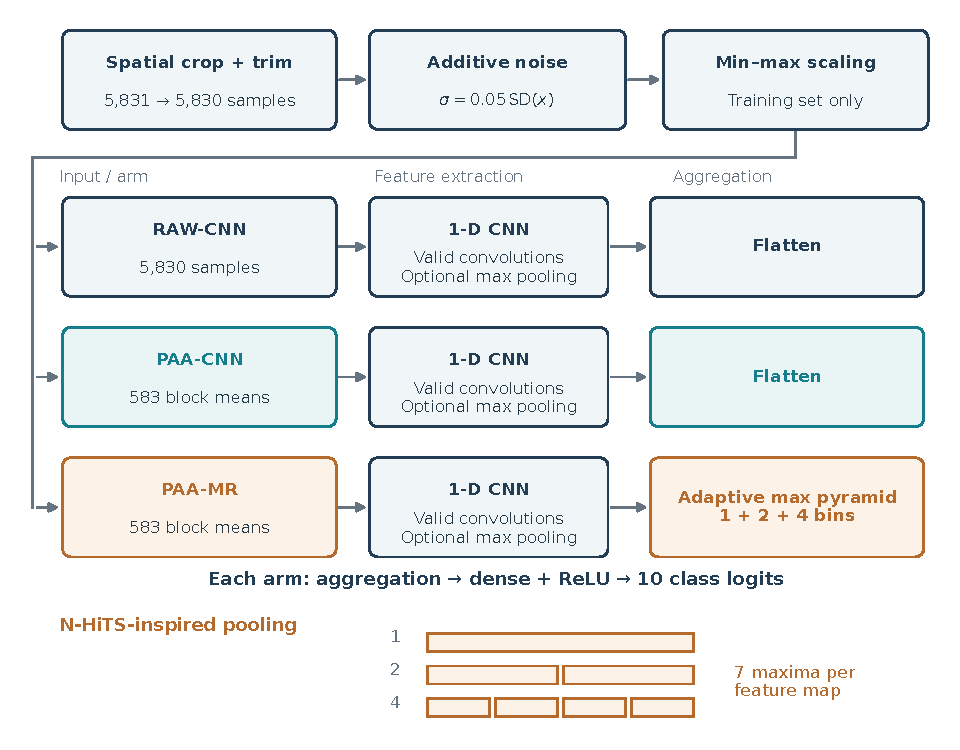
\includegraphics[width=0.92\textwidth]{f25_architecture.pdf}
\caption{Preprocessing and classifier arms of the F25 benchmark. RAW-CNN and
PAA-CNN flatten the last feature maps; PAA-MR replaces flattening with adaptive
max pooling at 1, 2, and 4 bins, giving seven values per feature map. All arms
end in a dense ReLU layer and ten class outputs.}
\label{fig:f25_architecture}
\end{figure}

\subsection{Hyperparameter optimization and training}

Hyperparameters are tuned by Bayesian optimization with the tree-structured
Parzen estimator~\cite{bergstra2011algorithms} implemented in
Optuna~\cite{akiba2019optuna}. As in the source, each optimization comprises
100 proposals, and each proposal is trained five times, here with fixed seeds;
the objective is the mean validation accuracy of the five runs. The search space
is that of the source: one to five convolutional layers, 32--128 filters in
steps of 16, kernel sizes of 2--5, optional max pooling after each layer, 16--64
dense units in steps of 16, batch sizes of 8--48 in steps of 8, and a learning
rate between $10^{-5}$ and $10^{-2}$, sampled on a logarithmic scale.

Networks are trained with the Adam optimizer~\cite{kingma2015adam} and the
cross-entropy loss. The learning rate is halved after 30 epochs without
improvement of the validation loss, down to $10^{-6}$; training stops after 50
epochs without improvement or at 1,000 epochs, and the weights with the lowest
validation loss are restored. These settings follow the source. The test set is
never used for tuning or for checkpoint selection. Each reported configuration
is finally trained with 20 initialization seeds that differ from the five
tuning seeds, and the complete 20-run distribution is reported. The models were
implemented in PyTorch~\cite{paszke2019pytorch} with deterministic GPU
algorithms.

\subsection{Experimental tiers}

F25-R tunes RAW-CNN and PAA-CNN separately for S00 and S01, as in the source.
F25-X comprises three tiers. In the frozen-single tier, the F25-R
hyperparameters tuned for the front bogie (S01) are applied to all six channels;
PAA-MR uses the PAA-CNN vector with only the pooling replaced. In the
tuned-single tier, each of the 18 arm--channel combinations receives its own
100-proposal optimization. In the frozen-pair tier, the frozen vectors are
applied to all 45 arm--pair combinations. The frozen tiers compare channels
under a common architecture, whereas the tuned tier compares them after
channel-specific tuning; a tuned--frozen difference therefore combines the
effect of tuning with the randomness of a finite search. The frozen S01 RAW-CNN
and PAA-CNN configurations repeat the F25-R ones and reproduce their results
exactly, so they are not additional evidence. In total, F25 comprises 22
optimizations and 85 reported configurations, that is, 11,000 tuning runs and
1,700 reported runs.

\subsection{Deviations from the source study}

F25-R is a publication-faithful reconstruction rather than an exact
replication. Table~\ref{tab:f25_deviations} lists the deliberate changes and
the choices that the publication does not report.

\begin{table}[htbp]
\centering
\caption{Differences between F25-R and the source study~\cite{fernandes2025early}.}
\label{tab:f25_deviations}
\small
\begin{tabular}{@{}>{\raggedright\arraybackslash}p{0.22\textwidth}
>{\raggedright\arraybackslash}p{0.33\textwidth}
>{\raggedright\arraybackslash}p{0.37\textwidth}@{}}
\toprule
Item & Source study & F25-R \\
\midrule
Deck mesh & 0.30~m; central support inside an element & 0.15~m uniform refinement; support on a node \\
Crack model & Tapered local $EI$ law~\cite{sinha2002simplified} & Uniform 22\% or 14\% $EI$ reduction over the same 0.30~m zone \\
Software & TensorFlow & PyTorch \\
Data split & Counts reported; allocation not reported & One seeded permutation shared by all scenarios \\
Min--max scaling & Calibration data not reported & Training set only, per channel \\
Learning-rate sampling & Range reported; distribution not reported & Logarithmic \\
Front-bogie finalist & Dense layer of 96 units, outside the reported 16--64 range & Search restricted to the reported range; the published finalists were not retrained \\
Monitoring window & 5,830 samples (58.3~m) & 5,831 inclusive samples, last one discarded \\
\bottomrule
\end{tabular}
\end{table}

\subsection{Performance metrics}

The main metric is the overall accuracy over the 1,000 test passages; with 100
test passages per scenario, it equals the mean recall of the ten scenarios.
Bearing, scour, and crack accuracies are obtained by mapping the predicted
scenario to its coordinates in Table~\ref{tab:f25_scenarios}: bearing damage
(present or absent), scour level (0, 5, or 10\%), and crack label (0, 5, or
10\%). They are projections of the ten-class prediction, not separately
trained classifiers. Confusion matrices are averaged over the 20 runs, with
rows denoting true scenarios. Means, sample standard deviations (SD), medians,
and seed-paired differences describe the variability caused by network
initialization for one fixed data partition; they are not confidence intervals
for other datasets or for field conditions. Because all configurations are
ranked on the same test set, rankings across channels and pairs are
exploratory, and the regression campaign does not use them to select its
response pair.

\section{F25 results and discussion}
\label{sec:f25_results}

All 22 optimizations completed their 100 proposals with five runs each, and all
85 configurations were trained with the 20 reporting seeds, giving 11,000
tuning runs and 1,700 reported runs. Every confusion matrix contains 100 test
passages per scenario. All reported accuracies were recomputed from the stored
confusion matrices, and the selected hyperparameters were checked against the
optimization databases. The simulations were run in MATLAB R2021a, and the
networks were trained on an NVIDIA GeForce RTX 2060 (6~GB) with PyTorch 2.6.0
and CUDA 11.8. The GPU driver was updated from version 591.86 to 610.88 during
the campaign, and one optimization was resumed after 65 of its 100 proposals;
the effect of the driver change was not quantified.

\subsection{Reconstruction of the source results}

Table~\ref{tab:f25_reconstruction} summarizes F25-R. The source study reports,
for each channel and input, the confusion matrix of the best of its 20
runs~\cite{fernandes2025early}; the corresponding accuracies, read from the
published figures, are therefore compared with the best of the present 20 runs
(column ``Max''). With RAW inputs, the best carbody run (71.8\%) exceeded the
published value (65.1\%), whereas the best front-bogie run (65.5\%) remained
below it (82.2\%). With PAA inputs, the best runs reached 66.6\% for the carbody
and 73.8\% for the front bogie, against the published 86.7\% and 82.1\%. The
benefit of PAA reported for the carbody sensor was reproduced in direction for
the mean (57.33\% for PAA against 49.74\% for RAW), but with a smaller
magnitude, and the best RAW run exceeded the best PAA run. On the front bogie,
PAA was the least stable configuration, with an SD of 21.30 percentage points
and three runs at 10\%.

\begin{table}[htbp]
\centering
\caption{F25-R ten-class test accuracy over 20 initialization seeds. SD is the
sample standard deviation in percentage points. The last column gives the
accuracy of the best of 20 runs in the source study, read approximately from
its published confusion matrices~\cite{fernandes2025early}.}
\label{tab:f25_reconstruction}
\small
% Generated by analyze_f25_results.py; source values are best-of-20 runs read from figures.
\begin{tabular}{llrrrr}
\toprule
Response & Input & Mean $\pm$ SD (\%) & Min (\%) & Max (\%) & Source, best run (\%) \\
\midrule
S00 & RAW & $49.74 \pm 12.86$ & 23.0 & 71.8 & 65.1 \\
S00 & PAA & $57.33 \pm 6.78$ & 41.5 & 66.6 & 86.7 \\
S01 & RAW & $49.41 \pm 11.60$ & 21.4 & 65.5 & 82.2 \\
S01 & PAA & $46.69 \pm 21.30$ & 10.0 & 73.8 & 82.1 \\
\bottomrule
\end{tabular}

\end{table}

The reconstruction gap cannot be attributed to a single cause. The crack
surrogate, the deck mesh, the software framework, the random partition, and
the optimization outcome all differ from the source
(Table~\ref{tab:f25_deviations}). The published front-bogie finalist, with a
96-unit dense layer, lies outside the reported search range, and the published
finalist architectures were not retrained. The validation objectives of the
F25-R optimizations (60.0--72.8\%) were also 8--26 percentage points higher
than the corresponding 20-run test means, a selection effect discussed in
Section~\ref{sec:f25_tuning}. The results therefore support an unresolved
reconstruction gap rather than a replication of the published accuracies.
The selected hyperparameters are listed in Table~\ref{tab:f25_hyperparameters};
the front-bogie vectors are the frozen hyperparameters of F25-X.

\begin{table}[htbp]
\centering
\caption{Hyperparameters selected by the 100-proposal searches for the F25-R
models and for the three tuned models on the carbody pitch rate (S05). Filters
are listed per convolutional layer; a superscript $p$ marks a layer followed by
max pooling.}
\label{tab:f25_hyperparameters}
\footnotesize
\setlength{\tabcolsep}{3pt}
\resizebox{\textwidth}{!}{% Generated by analyze_f25_results.py; winners of the 100-proposal searches.
\begin{tabular}{lllllrrrr}
\toprule
Study & Model & Channel & Filters & Kernels & Dense & Batch & Learning rate & Parameters \\
\midrule
F25-R & RAW-CNN & S00 & 112--48$^{p}$--112$^{p}$--48$^{p}$ & 2--5--5--4 & 48 & 40 & $9.8\times10^{-5}$ & 1,746,746 \\
F25-R & PAA-CNN & S00 & 80$^{p}$--128$^{p}$--64 & 3--5--5 & 64 & 40 & $3.2\times10^{-4}$ & 662,730 \\
F25-R & RAW-CNN & S01 & 96$^{p}$--32$^{p}$--48--96$^{p}$--32 & 2--4--5--4--5 & 64 & 32 & $5.9\times10^{-5}$ & 1,529,530 \\
F25-R & PAA-CNN & S01 & 112$^{p}$--112$^{p}$--96--32 & 2--5--3--3 & 64 & 48 & $4.9\times10^{-4}$ & 390,154 \\
F25-X tuned & RAW-CNN & S05 & 48$^{p}$--96--80$^{p}$ & 2--3--5 & 64 & 48 & $6.5\times10^{-5}$ & 7,497,738 \\
F25-X tuned & PAA-CNN & S05 & 64--80--128$^{p}$ & 3--5--3 & 48 & 32 & $8.8\times10^{-5}$ & 1,820,650 \\
F25-X tuned & PAA-MR & S05 & 32$^{p}$--64$^{p}$--32$^{p}$--80 & 2--3--3--5 & 32 & 48 & $4.7\times10^{-4}$ & 43,642 \\
\bottomrule
\end{tabular}
}
\end{table}

\subsection{Channel comparison under frozen hyperparameters}

Table~\ref{tab:f25_frozen_singles} and Fig.~\ref{fig:f25_singles}a compare the
six channels with the F25-R front-bogie hyperparameters. The carbody pitch rate
(S05) gave the highest mean in all three arms: $72.61\pm4.95\%$ for RAW-CNN,
$72.29\pm14.98\%$ for PAA-CNN, and $65.98\pm3.28\%$ for PAA-MR. The large SD of
PAA-CNN is caused by a single run at 10\%; the other 19 runs lay between 68.9\%
and 83.8\%. The vertical accelerations (S00--S02) gave intermediate results,
and the two bogie pitch rates (S06 and S07) stayed close to the 10\% chance
level in every arm. Under these frozen settings, multi-rate pooling did not
improve on the flatten-based arms.

\begin{table}[htbp]
\centering
\caption{F25-X ten-class test accuracy with frozen hyperparameters (mean
$\pm$ sample SD over 20 runs, \%). All arms use the F25-R front-bogie
hyperparameters; PAA-MR uses the PAA-CNN vector with multi-rate pooling.}
\label{tab:f25_frozen_singles}
\footnotesize
\setlength{\tabcolsep}{4pt}
\resizebox{\textwidth}{!}{% Generated by analyze_f25_results.py; percent mean +/- sample SD.
\begin{tabular}{llrrr}
\toprule
Code & Response & RAW & PAA & PAA-MR \\
\midrule
S00 & Carbody vertical & $51.10 \pm 10.47$ & $48.15 \pm 14.86$ & $22.38 \pm 1.34$ \\
S01 & Front-bogie vertical & $49.41 \pm 11.60$ & $46.69 \pm 21.30$ & $37.39 \pm 8.60$ \\
S02 & Rear-bogie vertical & $57.13 \pm 10.30$ & $51.40 \pm 20.48$ & $49.12 \pm 4.94$ \\
S05 & Carbody pitch rate & $72.61 \pm 4.95$ & $72.29 \pm 14.98$ & $65.98 \pm 3.28$ \\
S06 & Front-bogie pitch rate & $19.63 \pm 1.01$ & $15.16 \pm 4.40$ & $11.51 \pm 3.77$ \\
S07 & Rear-bogie pitch rate & $21.48 \pm 7.74$ & $13.23 \pm 4.70$ & $9.98 \pm 0.35$ \\
\bottomrule
\end{tabular}
}
\end{table}

The channel ranking has a plausible geometric explanation. The carbody pitch
responds to the difference between the vertical motions of the two bogies,
which are 16~m apart, a base comparable to the 19.95~m spans. It is therefore
sensitive to the slope of the deflected deck and to the support conditions.
This is the ``apparent profile'' mechanism through which McGeown et
al.~\cite{mcgeown2024pitch} detected pier scour from carriage pitch. The bogie
pitch, in contrast, responds to the difference between two wheelsets 2.3~m
apart, over which the long-wavelength deck deflection changes little; it is
dominated by the short-wavelength rail irregularity, which is identical in all
scenarios, and by the added noise, which scales with the standard deviation of
each signal. This interpretation is consistent with the results but was not
tested separately.

\subsection{Channel-specific tuning}
\label{sec:f25_tuning}

Channel-specific tuning changed both the accuracy and its variability
(Table~\ref{tab:f25_tuned_singles}, Fig.~\ref{fig:f25_singles}b). The highest
mean among the 18 tuned singles was obtained by PAA-MR on the carbody pitch
rate: $77.63\pm2.24\%$, with a median of 77.95\% and runs between 71.7\% and
81.1\%. Tuned PAA-CNN on the same channel reached the best single run
(88.0\%) and a similar median (77.45\%), but one run collapsed to 10\% and its
SD was 21.78 percentage points. PAA-MR/S05 has 43,642 trainable parameters,
against 1,820,650 for tuned PAA-CNN/S05 and 7,497,738 for tuned RAW-CNN/S05;
inference time and energy were not measured.

\begin{table}[htbp]
\centering
\caption{F25-X ten-class test accuracy after channel-specific tuning (mean
$\pm$ sample SD over 20 runs, \%). Each arm--channel combination has its own
100-proposal optimization.}
\label{tab:f25_tuned_singles}
\footnotesize
\setlength{\tabcolsep}{4pt}
\resizebox{\textwidth}{!}{% Generated by analyze_f25_results.py; percent mean +/- sample SD.
\begin{tabular}{llrrr}
\toprule
Code & Response & RAW & PAA & PAA-MR \\
\midrule
S00 & Carbody vertical & $60.06 \pm 8.38$ & $54.44 \pm 12.64$ & $35.73 \pm 12.90$ \\
S01 & Front-bogie vertical & $50.08 \pm 14.28$ & $70.05 \pm 8.96$ & $61.81 \pm 13.09$ \\
S02 & Rear-bogie vertical & $51.80 \pm 15.69$ & $68.61 \pm 2.52$ & $58.43 \pm 6.53$ \\
S05 & Carbody pitch rate & $70.95 \pm 14.74$ & $67.26 \pm 21.78$ & $77.63 \pm 2.24$ \\
S06 & Front-bogie pitch rate & $18.61 \pm 3.84$ & $21.62 \pm 13.13$ & $13.22 \pm 5.94$ \\
S07 & Rear-bogie pitch rate & $14.24 \pm 5.13$ & $19.35 \pm 6.32$ & $9.83 \pm 0.38$ \\
\bottomrule
\end{tabular}
}
\end{table}

\begin{figure}[htbp]
\centering
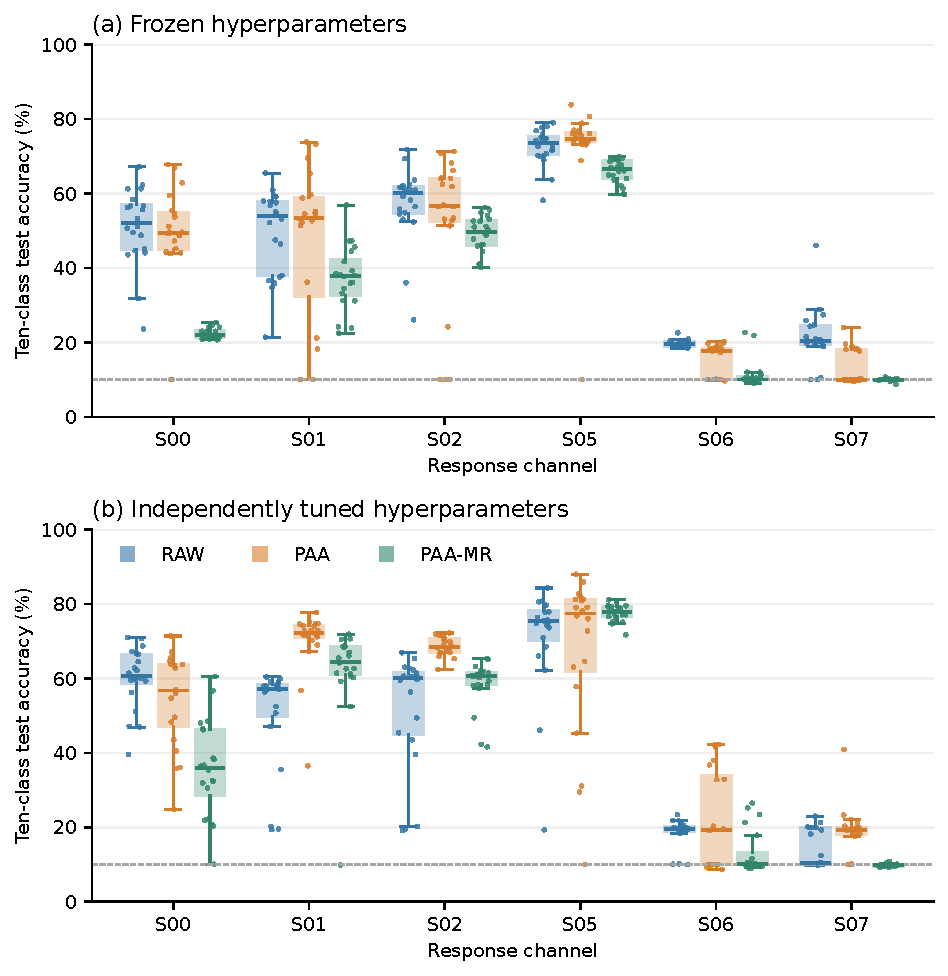
\includegraphics[width=0.92\textwidth]{f25_singles.pdf}
\caption{Distribution of the ten-class test accuracy of the six single channels
over 20 runs: (a) frozen hyperparameters; (b) channel-specific tuning. Boxes
show the median and interquartile range, whiskers extend to 1.5 times the
interquartile range, and dots show individual runs. The dashed line marks the
10\% chance level. All runs use the same passages and data partition.}
\label{fig:f25_singles}
\end{figure}

Tuning did not improve every configuration. For PAA-MR/S05, the seed-paired
gain over the frozen configuration was $+11.65$ percentage points (SD of the
paired differences 3.64), and all 20 runs improved. In contrast, the mean
accuracy of PAA-CNN/S05 decreased by 5.03 points and that of RAW-CNN/S07 by
7.25 points. Part of this behaviour is a selection effect. Each optimization
selects the best of 100 proposals on only 200 validation passages, and five
runs per proposal rarely reveal failures that occur in about one of 20
initializations. Across the 22 tuned configurations, the validation objective
of the selected proposal exceeded the subsequent 20-run test mean by 10.5
percentage points on average (range 1.4--26.1). For the S05 winners, the
validation objectives were 84.5\% (RAW-CNN), 83.5\% (PAA-CNN), and 79.4\%
(PAA-MR), against test means of 70.95\%, 67.26\%, and 77.63\%. PAA-MR/S05 thus
had the smallest optimism among the informative channels. Because all
configurations are compared on the same test set, the best configuration was
identified after the test results were known; the ranking is descriptive.

\subsection{Two-channel inputs}

Fig.~\ref{fig:f25_pairs} shows the mean accuracy of all 45 frozen pairs, and
Table~\ref{tab:f25_pairs} lists the three best pairs of each arm. All of them
contain the carbody pitch rate. A second channel rarely improved on the better
of its two members. The highest pair mean, $75.68\pm4.59\%$ for PAA-CNN with
S00+S05, exceeded the frozen PAA-CNN/S05 mean (72.29\%) only because of the
collapsed single-channel run: both medians are 74.55\%, and, paired by seed,
the pair was more accurate in only 9 of the 20 runs. For RAW-CNN, the S00+S05
pair reached $71.69\pm8.54\%$, against $72.61\pm4.95\%$ for S05 alone, and 11
of the 15 pairs had a lower mean than their better member. The only top-ranked
pair with a consistent gain was S02+S05 with PAA-MR: $70.63\pm5.16\%$, 4.65
points above PAA-MR/S05, with higher accuracy in 15 of the 20 paired runs. The
pairs were not tuned, so these comparisons concern a fixed architecture; they
are exploratory and were not used to select inputs for the regression campaign.

\begin{figure}[htbp]
\centering
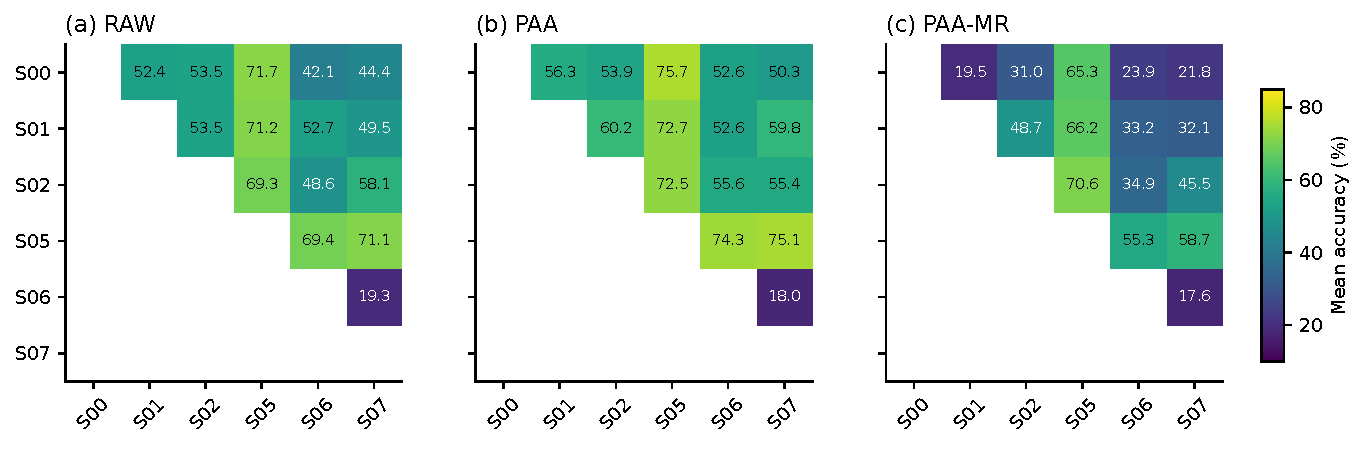
\includegraphics[width=\textwidth]{f25_pairs.pdf}
\caption{Mean ten-class test accuracy (\%) over 20 runs of the 15 two-channel
inputs with frozen hyperparameters: (a) RAW-CNN; (b) PAA-CNN; (c) PAA-MR.}
\label{fig:f25_pairs}
\end{figure}

\begin{table}[htbp]
\centering
\caption{Three best two-channel inputs of each arm with frozen hyperparameters
(ten-class test accuracy over 20 runs, \%). The ranking is exploratory.}
\label{tab:f25_pairs}
\small
% Generated by analyze_f25_results.py; exploratory test-read rankings.
\begin{tabular}{llrr}
\toprule
Arm & Response pair & Mean $\pm$ SD (\%) & Median (\%) \\
\midrule
RAW & S00+S05 & $71.69 \pm 8.54$ & 73.10 \\
RAW & S01+S05 & $71.20 \pm 6.83$ & 73.45 \\
RAW & S05+S07 & $71.12 \pm 5.36$ & 72.90 \\
PAA & S00+S05 & $75.68 \pm 4.59$ & 74.55 \\
PAA & S05+S07 & $75.08 \pm 3.60$ & 75.30 \\
PAA & S05+S06 & $74.28 \pm 6.40$ & 73.75 \\
PAA-MR & S02+S05 & $70.63 \pm 5.16$ & 71.65 \\
PAA-MR & S01+S05 & $66.17 \pm 10.69$ & 67.40 \\
PAA-MR & S00+S05 & $65.33 \pm 7.09$ & 67.75 \\
\bottomrule
\end{tabular}

\end{table}

\subsection{Discrimination of damage types}

For tuned PAA-MR/S05, the mean accuracies of the three damage coordinates were
99.97\% for the bearing condition, 97.63\% for the scour level, and 77.76\% for
the crack label. The corresponding majority-class rates are 60\%, 40\%, and
50\%, because the catalogue is not balanced along each coordinate. Bearing
damage and scour level were thus recognized almost perfectly from a single
carbody channel, and the crack label limited the overall accuracy.

The mean confusion matrix (Fig.~\ref{fig:f25_confusion}) shows this structure
directly. All eight off-diagonal entries above 10\% involve pairs of scenarios
that differ only in the crack coordinate: Healthy and DC2 (31.8\% and 24.1\%),
DC4 and DC7 (15.7\% and 14.9\%), DC5 and DC8 (19.2\% and 17.2\%), and DC9 and DC10
(37.5\% and 39.6\%). The two scenarios whose combination of scour level and
bearing condition is unique in the catalogue, DC3 and DC6, were recognized in
89.8\% and 99.1\% of the cases. The DC9/DC10 pair, which differs only in crack
severity, was also the main source of error in the published carbody results of
the source study~\cite{fernandes2025early}. Within this catalogue, a local
$EI$ reduction of 14--22\% over 0.30~m is thus much harder to recognize from the
vehicle response than a 5\% loss of support stiffness or the restraint of an
end bearing. This conclusion is conditional on the crack surrogate and its
single location.

\begin{figure}[htbp]
\centering
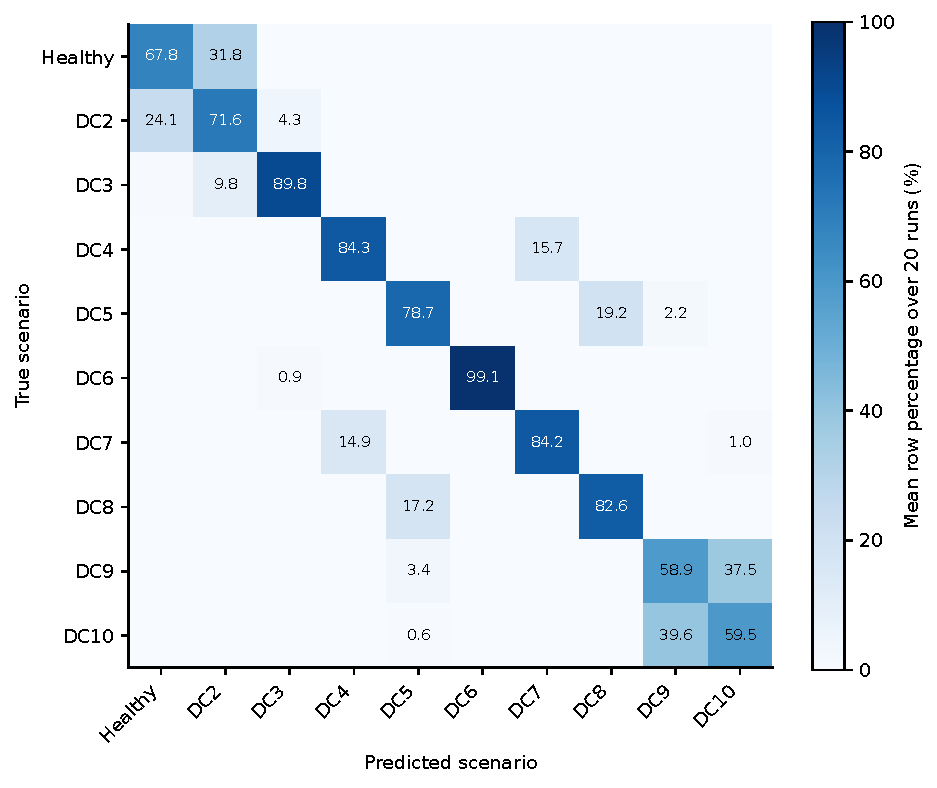
\includegraphics[width=0.82\textwidth]{f25_confusion.pdf}
\caption{Confusion matrix of tuned PAA-MR on the carbody pitch rate (S05),
averaged over the 20 runs; rows are true scenarios and entries are row
percentages. Entries below 0.5\% are not labeled.}
\label{fig:f25_confusion}
\end{figure}

\subsection{Training stability}

Of the 1,700 reported runs, 90 predicted a single class for every test passage
and 132 had an accuracy of 10\% or less. Sixty of the 90 single-class
collapses used one of the two bogie pitch rates, which are close to chance
level in any case. Excluding these single-channel configurations, single-class
collapses occurred in
26 of 500 PAA-CNN runs, 3 of 500 RAW-CNN runs, and 1 of 460 PAA-MR runs; these
counts include the two repeated F25-R control configurations. In addition, 379
runs restored a checkpoint from epoch 950 or later, 53 of them at epoch 1,000,
so the 1,000-epoch limit of the source protocol was active in part of the
runs. All runs are kept in the reported distributions. The frequency of
collapsed runs shows why a single best run, or a mean without the
distribution, is an incomplete summary of a drive-by classifier.

The F25 results concern ten fixed scenarios, one bridge, one rail profile, and
a passage-level split. They provide no evidence on continuous scour
estimation, unseen damage states, measured signals, or other rail profiles;
the four-block regression results remain pending in the next section.

\section{Pending four-block regression results and discussion}
\label{sec:results}

% =====================================================================
% HARD RULE (do not remove until the campaign is complete):
% This section excludes the separate, completed F25 classification evidence.
% Populate this section ONLY from authenticated outputs of the complete
% four-block Paper-1 campaign at the clean campaign source commit. No number,
% figure, ranking, or qualitative outcome from a pilot or superseded design is
% admissible, even as a placeholder.
% =====================================================================

\subsection{Campaign accounting and local qualification}
\label{sec:accounting}

This subsection will identify the campaign source revision, protocol and
source-root digests, recorded generation and training environments, per-PC
capability/physics-smoke and CUDA-capacity results, rail-clearance and
response-sensitivity verdicts, contact/time-step closure, and exact artifact
inventories. It will
confirm 305/425/475/475 states and 50 passages per state for
F40-S/F40-M/L99-S/L99-M, respectively, and document that no failed, incomplete,
retried, out-of-memory, provenance-inconsistent, or post-contact-violation job
entered a reported result.
\pending{Complete accounting from the authenticated campaign artifacts,
including all 160 primary HPO studies, 1,440 planned primary refits, and
sealed-test openings.}

\subsection{F40-S architecture-factorial adjudication}
\label{sec:factorial_results}

The F40-S front-bogie anchor table will report all 16 registered cells,
crossing input representation, position encoding, LSTM, and multi-rate pooling. For each
cell, five 100-trial HPO winners are adjudicated by one complete three-fold
grouped-development OOF partition and two initialization seeds. Tables will
show the paired state-clustered OOF scour MSE used for selection, the selected
restart vector, and the best RAW and PAA cells. Outer-test values are excluded
from these selection tables by construction.
\pending{Authenticated 16-cell Option-C OOF table and selected RAW/PAA cells;
report ties using the prospectively fixed restart-seed and cell-ID rules.}

\subsection{Response-channel screen and selected pair}
\label{sec:selection_results}

For each of the four retained slots --- best RAW, best PAA, RAW CNN--GAP, and
PAA CNN--GAP, with authenticated alias deduplication --- the frozen F40-S
screen uses five paired initialization seeds. The eight-response payload is
retained, but wheelset
proxy indices 3 and 4 are diagnostic-only and never enter a fit. The eligible
screen therefore contains six non-selectable singles and 15 selection-eligible
pairs. Pair selection averages state-level scour MSE across seeds, validation
states, and unique resolved pipelines, with lexicographic ascending-pair
tie-breaking. The full tensor, coverage, and deduplication map will accompany
the selected pair.
\pending{Authenticated 420-job channel-screen table, single-channel diagnostics,
resolved-pipeline map, and selected physical two-channel pair.}

\subsection{Block-local selected-pair performance and stability}
\label{sec:block_results}

The selected pair is re-optimized for the four retained slots in F40-S and
independently in F40-M, L99-S, and L99-M. Primary tables will report scour MSE
in squared percentage points (aggregate and per support, with RMSE where
useful), post-freeze distributions across 30 disjoint initialization seeds per
slot and block, and the prospectively frozen comparator set. These 480
sealed-test stability fits are report-only: they cannot change a selected
pipeline, pair, hyperparameter vector, or checkpoint policy.
\pending{Authenticated block-local HPO winners and sealed-test estimates for
the resolved RAW/PAA winners and CNN--GAP baselines in all four blocks.}

Any secondary contemporary-architecture results are admitted only after this
screen and use the exact authenticated primary F40-S pair. ModernTCN- and
TSLANet-inspired challengers have no independent pair-selection path and cannot
change the primary factorial, screen, or selected pair.

\subsection{Multi-pier estimation, localization, and bearing leakage}
\label{sec:multipier_results}

For L99-S and L99-M, results will separate aggregate from support-specific
scour error and report parity plots for supports 2--4. Most-affected-support
localization is the registered passage-level estimate restricted to passages
whose maximum true scour exceeds 5 percentage points. For F40-M and L99-M,
bearing-head error, false scour response in bearing-only states, and false
bearing response in scour-only states will be reported separately from scour
performance.
\pending{Per-support estimation, localization, bearing-head, and
scour--bearing leakage results from authenticated sealed-test artifacts.}

\subsection{Paired S--M comparisons}
\label{sec:paired_results}

The two registered cross-block comparisons have different pairing scopes.
F40-S versus F40-M uses only their 30 shared controlled semantic states;
L99-S versus L99-M uses all 475 shared states. In each case the S--M change
jointly activates nominal bearing-fixity physics, local $EI$ loss, and bearing
heads/multi-task learning, so it is reported as a combined model/task contrast,
not an isolated bearing or crack effect. State-first paired summaries use only
authenticated shared identities and preserve the finite-design, descriptive
claim boundary.
\pending{Authenticated F40 and L99 paired S--M effects with explicitly
descriptive finite-design uncertainty summaries.}

\subsection{F40 classification comparability check}
\label{sec:classification_results}

The F40-S regression dataset also supplies the predeclared 0, 5, 10, and 20\%
severity subset used for a Fernandes-style classification comparability check.
With five semantic replicas per class, this arm is deliberately secondary and
is not treated as a headline estimate or an exact replication.
\pending{Authenticated classification-comparability results and their deviation
statement; do not import published targets as observed results of this study.}

\subsection{Model-form sensitivities}
\label{sec:model_form_results}

Before physical interpretation, the manuscript will report the prospective
one-seat/two-rail parameter scaling, 0.545-to-0.600~m spacing recalculation,
rail-damping-target, and fixed-healthy-Rayleigh sensitivities. The inherited
ballast-shear/condensation topology has no sensitivity arm and remains an
explicit limitation. These analyses qualify the model form; they do not select
the neural architecture or admit a new production configuration after freeze.
\pending{Authenticated model-form sensitivity estimates and the resulting
pre-freeze production verdicts.}

\subsection{Secondary frozen transfer}
\label{sec:transfer_results}

F40-S settings are additionally evaluated without block retuning on each of
the three downstream blocks for four slots and five initialization seeds (60
fits). These rows are descriptive, labeled secondary/non-selection, and kept
separate from the independently tuned primary block results.
\pending{Authenticated secondary frozen-transfer results, reported without a
transport or rescue claim.}

\subsection{Discussion}
\label{sec:discussion}

The discussion will be limited to authenticated estimates. It will address
whether RAW or PAA and each factorial component changes observed error under
the matched search budget; which eligible modeled-DOF response pair the F40-S
screen selects and what the diagnostic-only wheelset-proxy boundary implies;
whether the
four retained pipelines behave consistently after independent block-local
tuning; how multi-pier and bearing-aware tasks change errors; and how sensitive
the interpretation is to the registered track/damping model-form choices.
Cross-geometry patterns and frozen transfer will remain descriptive, and no
result will be generalized to field sensors, unseen profiles, or deferred
track/train damage.
\pending{Discussion grounded only in authenticated four-block estimates.}

\section{Limitations and practical feasibility}
\label{sec:limitations}

The claims supported by this study are bounded by its physical model,
observation model, and finite registered design. We state those boundaries
explicitly before discussing field deployment.

The completed F25 classification evidence and the prospective four-block
regression campaign have different statistical scopes. Statements below about
four-block selection, qualification, stability, and paired comparisons describe
the prospective protocol; their outcomes remain pending.

\subsection{Scope of the completed F25 evidence}

F25 holds out passages within ten fixed structural classes. It evaluates
recognition of those configurations under operational variation, not unseen
damage states, crack locations, profiles, or field observations. The 20-seed
standard deviations describe initialization variability on one partition and
are not population confidence intervals. Frozen singles, separately
reoptimized singles, and exploratory frozen pairs answer different questions.
Their observed test-table maxima do not authorize a new selected model or
pair, and a best-run confusion matrix is a visual diagnostic rather than a
distributional estimate. Comparisons to published confusion-matrix readings
are approximate and affected by the documented reconstruction deviations.
RAW/PAA changes can also alter flatten-based model capacity; an accuracy
difference does not isolate compression alone. Ten-class accuracy and
damage-axis accuracy do not measure open-set detection, calibrated damage
probabilities, or performance on a population of real bridges.

\subsection{Physical model and label semantics}

\begin{itemize}
  \item \textbf{Simulation only.} All responses are generated by the registered
  TTBI model; no field measurement enters the study. Every conclusion is
  conditional on this simulated distribution.

  \item \textbf{Two-dimensional vertical dynamics.} The model captures
  vertical and pitch response only. Lateral, torsional, soil-continuum, and
  pier-tilt behaviour --- all potentially informative for scour --- are absent.

  \item \textbf{The support spring is not soil--structure interaction.} One
  vertical spring per bridge support represents the foundation. The target is
  modeled support-stiffness loss in percentage points, not scour depth,
  embedment loss, or eroded volume; no universal hydraulic-to-stiffness mapping
  is claimed.

  \item \textbf{Bearing and crack labels are design coordinates.} Nominal
  abutment rotational fixity is not a calibrated physical bearing-condition
  percentage. The crack arm is a uniform local finite-element $EI$ reduction,
  not a breathing crack or calibrated crack-depth model
  \cite{sinha2002simplified}.

  \item \textbf{One fixed rail profile and restricted nuisance scope.}
  One generated FRA-class-4 profile realization is shared by all semantic
  states and passages. Rail-profile phase is therefore not an EOV in this
  experiment, and performance is conditional on that realization. The study
  supports no claim of robustness or transport to alternative phases, measured
  profiles, or unseen track sections. Track-layer damage, wheel
  polygonization, and suspension damage are disabled.

  \item \textbf{The nominal track is an inherited simplified topology.} The
  planar source combines two-rail quantities for rail inertia/mass and a full
  sleeper, but retains other values that Zhai et al.~\cite{zhai2004track}
  report per rail seat. It also retains source values derived at 0.545~m on a
  0.600~m support lattice, omits the adjacent-ballast $K_w,C_w$ shear branch,
  and condenses each on-bridge ballast lump onto the support-aligned deck node.
  The production baseline is therefore neither a demonstrated one-seat model
  nor a consistently doubled two-rail model, and it is not a complete Zhai
  reproduction. Prospective one-seat/two-rail and 0.545-to-0.600~m
  parameter-transfer sensitivities quantify two parameter-level choices; the
  omitted-shear/condensation topology itself remains unexamined. The wheelset
  proxies are retained only for physical diagnostics and are excluded from
  learning, so they cannot win the channel selection or support a headline
  sensor result.

  \item \textbf{Damping is model-form dependent.} The 0.1\% rail Rayleigh
  target is an inherited author-chosen value, not a property reported by Zhai;
  a prospective damping sensitivity bounds that choice. Production recomputes
  bridge coefficients for each realized state and recomputes them separately
  on every mesh in refinement studies, with rail damping referenced to the
  corresponding bridge modes. A fixed-healthy/fixed-grid coefficient arm is a
  model-form sensitivity. Consequently, stiffness interventions in the
  production model alter both assembled stiffness and Rayleigh-dependent
  damping; they are not evidence for physical damage-dependent damping.

  \item \textbf{Bilateral contact.} The linear wheel--rail model does not
  simulate separation and re-contact. The authenticated contact gate aborts
  generation on registered violations, but passing that gate does not quantify
  the response error caused by the bilateral approximation.

  \item \textbf{Author-chosen operational design.} The speed and temperature
  envelopes, deck-modulus temperature law, and vehicle-property perturbations
  were not fitted to a route, climate, or fleet population. Results are
  conditional on those finite design choices.
\end{itemize}

\subsection{Observation model and channel-level claims}

\begin{itemize}
  \item \textbf{Noise is a symmetric stress, not a hardware model.} The 5\%
  relative-noise arm applies the same mathematical rule to every channel and
  includes no transducer noise density, bias stability, bandwidth, mounting
  transfer function, or environmental qualification.

  \item \textbf{Channels are not sensors.} The experiment ranks modeled
  responses, not physical transducer counts or placements. In particular, the
  eight-response \texttt{physical8\_v1} payload includes two total
  constrained-motion wheelset proxies assembled from the linear model. They are
  kinematic diagnostics, not sensors or independent degrees of freedom, and are
  excluded from every learning and selection input. They also omit axle-box
  mounting dynamics, local wheel/rail compliance beyond the model, sensor
  bandwidth and filtering, and contact nonlinearity. They must not be described
  as measured axle-box accelerations without a separate observation model.
\end{itemize}

\subsection{Statistical scope}

\begin{itemize}
  \item \textbf{Conditional finite-budget selection.} ``Best'' means best
  under the registered 16-cell search space, HPO budgets, fixed folds, seed
  lists, and F40-S channel screen. Equal budgets do not eliminate finite-search
  optimization error, and no global architecture or sensor optimum is claimed.

  \item \textbf{Development adjudication is selection, not stability.} The
  480 Option-C out-of-fold fits choose the F40-S vectors and therefore cannot
  estimate post-selection stability. Stability is reported separately from 30
  disjoint post-freeze initialization seeds per retained pipeline and block on
  the sealed outer test; those runs cannot re-rank a model.

  \item \textbf{The channel screen has an asymmetric role.} Six eligible singles are
  reported but non-selectable; only the 15 eligible pairs can win. Subsequent HPO on the
  selected pair may improve its block-local model but is not evidence that the
  pair beats the other 14 pairs that were screened under frozen F40-S settings.
  Any contemporary challenger enters only afterward on this same authenticated
  pair and has no independent channel-selection claim.

  \item \textbf{Descriptive uncertainty, not population coverage.} State-first
  resampling and across-seed summaries are finite-design sensitivity analyses.
  They are not confidence intervals for a field population, familywise-error
  controlled tests, or guarantees of statistical significance or superiority.

  \item \textbf{Independent tuning changes the cross-block estimand.} Primary
  results compare pipelines after block-local HPO. They do not estimate
  zero-shot transfer. Frozen F40-S settings are evaluated downstream only in a
  separately labelled, secondary non-selection analysis.

  \item \textbf{Execution hosts are heterogeneous by design.} Production runs
  are admitted by capability and local qualification rather than by an exact
  software pin: GPU model, CUDA/PyTorch build and MATLAB release may differ
  between machines, and their exact identities are retained only as
  provenance. Two registered controls bound what that can affect. Training
  jobs are allocated to machines by seed-index parity, identically for every
  compared pipeline, so each allocation seed resolves to a single machine and
  every contrast paired on that seed is formed within one host. Each
  generation stage is produced entirely under one MATLAB environment, because
  a run folder can be resumed only under its recorded release and environment
  digest. Consequently no result reported here is claimed to be bitwise
  reproducible across machines, and absolute error magnitudes may carry a
  small host-dependent component. Only the paired within-block contrasts are
  protected from it, which is a further reason---beyond the independent tuning
  above---that cross-block comparisons are reported descriptively.

  \item \textbf{No detection claim from the regression protocol.} The
  prospective four-block study reports continuous regression
  error and localization. Sensitivity, specificity, probability of detection,
  calibrated damage probability, and minimum detectable severity would require
  a development-selected decision threshold that this protocol does not define.
\end{itemize}

\subsection{Practical feasibility and implementation challenges}

Field use first requires a hardware-specific observation model. Transducers,
mounts, acquisition chains, and environmental loads differ markedly across a
vehicle; axle-box environments are especially demanding~\cite{en61373}.
Second, supervised deployment requires trustworthy labels or a credible route
through model updating, domain adaptation, or hybrid physics--data methods.
The simulation-to-field gap --- model-form error, unmodeled EOVs, traffic
variability, and asset variability --- remains the dominant unquantified risk
\cite{malekjafarian2015review, fernandes2026canelas}. Third, the spatial
transform assumes known passage speed and repeated passages require fleet and
positioning integration. Finally, the prospective regression models cover one
train class and two idealized bridge geometries, while F25 uses its separate
two-span benchmark. Transfer across vehicles, bridge types, profiles,
and speeds outside 70--90~km/h is untested. A staged pathway should therefore
begin with instrumented healthy crossings for EOV and observation-model
calibration, followed by controlled stiffness interventions or monitored
scour-critical structures.

\section{Conclusion}
\label{sec:conclusion}

The completed F25 reconstruction and extension provide classification evidence
for ten prescribed bridge-damage configurations under operational variation.
In the separately reoptimized F25-X single-channel table, PAA with multi-rate
pooling on carbody pitch rate achieved $77.63\%$ mean test accuracy with a
$2.24$ percentage-point standard deviation over 20 initialization seeds. In the
exploratory frozen-hyperparameter pair table, PAA-CNN using carbody pitch rate
and carbody vertical acceleration achieved a mean of $75.68\%$ with a $4.59$
percentage-point standard deviation. These are descriptive summaries of
different analysis tiers; the latter is not a selected pair for the
four-block regression campaign. Comparisons remain conditional on one
partition, one profile, the specified search budget, and the modeled
observation channels.

F25 is a publication-faithful reconstruction rather than an exact replication.
Its support-aligned mesh, local uniform-$EI$ crack surrogate, software
framework, and explicitly assigned seeds impose documented deviations.
Passage-level test performance measures recognition of the ten fixed
configurations under new operational draws, not generalization to unseen
structural states. The class labels combine three damage axes and do not form
a single ordinal severity scale.

The prospective four-block framework addresses the separate question of
continuous support-stiffness-loss estimation on held-out structural states.
It specifies F40-S, F40-M, L99-S, and L99-M; semantic state grouping and
common-random-number pairing where catalogues overlap; a sealed outer test;
grouped-development out-of-fold adjudication; a fixed channel screen;
independent selected-pair optimization in each block; and disjoint report-only
initialization seeds. F25 results do not complete those analyses.

\pending{Summarize authenticated four-block outcomes after execution: RAW/PAA
factorial winners, selected pair, block-local scour performance and stability,
multi-pier localization, bearing leakage, and paired S--M comparisons.}

Both experiments remain simulation studies. Their modeled response channels
are not validated transducer packages, the wheelset proxies are excluded from
learning, and the stiffness-loss labels are not scour depth. Field deployment
requires measured crossings, a hardware-specific observation model, alternative
track profiles, and explicit evaluation of the simulation-to-field gap.


\section*{Acknowledgments}
% TBD: advisors (UFSC / UCSD), computing resources, discussion partners.

\subsection*{Author Contributions}
% TBD.

\subsection*{Funding}
% TBD (e.g., CAPES/CNPq sandwich scholarship --- fill in the grant program and number).

\subsection*{Conflicts of Interest}
The author(s) declare(s) that there is no conflict of interest regarding the
publication of this article.

\subsection*{Data Availability}
% Registered plan: release the campaign manifests (protocol descriptors, split
% manifests, HPO/champion manifests, execution receipts) and the analysis
% tables alongside the code repository; raw MATLAB time histories available on
% request due to size. Fill in the archive DOI at submission.
\pending{data archive DOI and released-artifact list}

\printbibliography

\end{document}
